\documentclass{beamer}

\usetheme{CambridgeUS}

\usepackage[utf8x]{inputenc}
\usepackage{tabularx}
\usepackage[romanian]{babel}
\usepackage{natbib}
\usepackage{bibentry}
\usepackage{amsmath}
\usepackage{mathtools}
\usepackage{algorithm}
\usepackage{algorithmic}
%\usepackage{algorithmicx}
%\usepackage[compatible]{algpseudocode}
\usepackage{graphicx}
\usepackage{caption}
\usepackage{subcaption}
\usepackage{multicol}

%\usepackage[framed,numbered,autolinebreaks,useliterate]{mcode}
\usepackage[nodisplayskipstretch]{setspace}
\setstretch{0.75}

\title[ARIA]{Modele Markov Ascunse}

\subtitle{De la Teorie la Aplicații}

\author[A. Sorici, T. Berariu]{Alexandru Sorici, Tudor Berariu}

\institute[AI-MAS]{Asociația Română pentru Inteligență Artificială}

%% TODO de pus frumos titlurile secțiunilor


%% Pentru a pune contents si frame cu titlu pe part
\makeatletter 
\AtBeginPart{%
\addtocontents{toc}{\protect\beamer@partintoc{\the\c@part}{\beamer@partnameshort}{\the\c@page}
  }%
  % \begin{frame}
  %   \center{ 
  %     \Large{
  %       \beamer@partname 
  %     }
  %   }
  % \end{frame}
  \begin{frame}{Outline}
    \tableofcontents[currentpart]
  \end{frame}
}


%% number, shortname, page.
\providecommand\beamer@partintoc[3]{%
  \ifnum\c@tocdepth=-1\relax
  % requesting onlyparts.
  \center{
  \makebox[20em]{PART #1.} \makebox[20em]{\Large{\textbf{#2}}}
}
  \par
  \fi } 

\define@key{beamertoc}{onlyparts}[]{%
  \c@tocdepth=-1\relax } \makeatother%


%% pentru a pune inainte de fiecare sectiune
\AtBeginSubsection[] {
  \begin{frame}{Outline}
    \tableofcontents[currentsection,currentsubsection,hideallsections]
  \end{frame}
}


\begin{document}
\maketitle

%\abovedisplayskip=8pt
%\belowdisplayskip=8pt
%\abovedisplayshortskip=2pt
%\belowdisplayshortskip=2pt


\begin{frame}
  \tableofcontents[onlyparts]
\end{frame}

\begin{frame}
  \frametitle{Outline}
  \tableofcontents[pausesections]
\end{frame}

\section{Aplicații în Învățarea Automată pentru MMA}
\label{sec:intro-to-hmm}

\subsection{Învățarea Automată}
\label{sec:machine-learning}

%% tudorel
\begin{frame}
  \frametitle{Ce este Învățarea Automată?}
  \begin{block}{Învățarea automată}
    Un program se spune că învață dintr-o mulțime de experiențe $E$
    relativ la o clasă de task-uri $T$ și o măsură a performaneței $P$
    dacă performața acestuia la execuția task-urilor $T$, măsurată de $P$,
    se îmbunătățește în urma experiențelor $E$.
    \citep{Mitchell:1997:ML:541177}
  \end{block}
\end{frame}

\begin{frame}[t]
  \frametitle{Aplicații ale Învățării Automate}
  \begin{itemize}
  \item \alert<1>{Self-Driving Car: Google Car}
  \item \alert<2>{Traducere Automată: Google Translate}
  \item \alert<3->{Sisteme de Recomandare}
    \begin{itemize}
    \item \alert<3>{Filme: ImDB, NetFlix}
    \item \alert<4>{Publicitate Inteligentă: Google Ads, Facebook Ads}
    \end{itemize}
  \end{itemize}
  \begin{center}%
    \only<1>{\includegraphics[width=0.5\textwidth]{graphics/ml-intro/google-car}}%
    \only<2>{\includegraphics[width=0.9\textwidth]{graphics/ml-intro/translate}}%
    \only<3>{\includegraphics[width=0.65\textwidth]{graphics/ml-intro/recommender}}%
    \only<4>{\includegraphics[width=0.65\textwidth]{graphics/ml-intro/advertizing}}%
  \end{center}
\end{frame}

\begin{frame}[t]
  \frametitle{Învățarea Automată: Tipuri de probleme}
  \begin{block}{Tipuri de probleme}
    \begin{itemize}
    \item Regresie
      \begin{itemize}
      \item predicția evoluției prețului unui bun
      \end{itemize}%
      \only<3->{
      \item Clasificare
        \begin{itemize}
        \item clasificarea obiectelor dintr-o imagine\\
          (imagine de la  Albert-Ludwigs-Universität, 
          Lehrstuhl für Mustererkennung und Bildverarbeitung)
        \end{itemize}
      }%
      \only<5->{%
      \item Învățare prin Recompensă
        \begin{itemize}
        \item jucător inteligent pentru backgammon
        \end{itemize}
      }%
    \end{itemize}
  \end{block}%
  \begin{center}
    \only<1>{\includegraphics[width=.6\textwidth]{graphics/ml-intro/ml-1}}%
    \only<2>{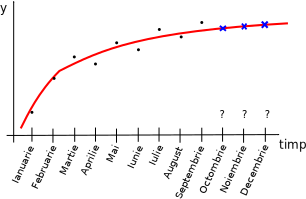
\includegraphics[width=.6\textwidth]{graphics/ml-intro/ml-2}}%
    \only<3>{\includegraphics[width=.35\textwidth]{graphics/ml-intro/car-2}}%
    \only<4>{\includegraphics[width=.35\textwidth]{graphics/ml-intro/car-1}}%
    \only<5>{\includegraphics[width=.28\textwidth]{graphics/ml-intro/backgammon}}%
  \end{center}
\end{frame}

\begin{frame}
  \frametitle{Tipuri de învățare}
  \begin{block}{Învățare Supervizată}
    \alert{Învățarea supervizată} se face pe baza unor date de antrenare etichetate.
    \begin{itemize}
    \item construirea unui model climatic pe baza datelor din utimii 30 de ani (regresie)
    \item construirea unui detector de mesaje spam (clasificare)
    \end{itemize}
  \end{block}\pause
  \begin{block}{Învățare Nesupervizată}
    În \alert{învățarea nesupervizată} nu există date etichetate.
    \begin{itemize}
    \item detectarea profilurilor de comportament ale cumpărătorilor
    \end{itemize}
  \end{block}
\end{frame}

\subsection{MMA în Învățarea Automată}
\label{sec:hmm-in-ml}

%% alejandro

%% aici facem tranzitie de la problema generala de ML
%% la probleme cu secvente temporale, markov stuff, dbn shit
%% adica HMM-uri :))

%% Markov models, Dynamic Bayesian Networks
\begin{frame}
  \frametitle{Probleme cu Secvențe Temporale (I)}
  \only<1>{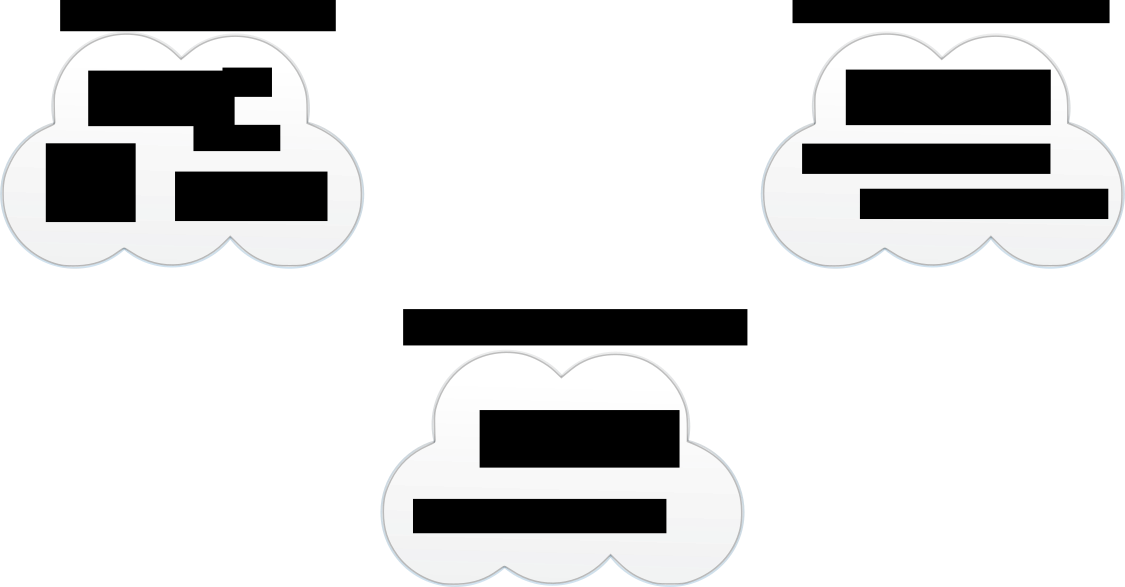
\includegraphics[width=\textwidth]{graphics/hmm-intro/time_series_problems_1.pdf}}
  \only<2>{
  	\includegraphics[width=\textwidth]{graphics/hmm-intro/time_series_problems_1_2.pdf}
  	\footnote{Sursa imaginii: Navstar}
  }
  \only<3>{
  	\includegraphics[width=\textwidth]{graphics/hmm-intro/time_series_problems_1_3.pdf}
  	\footnote{Sursa imaginii: http://www.hapblog.com/2012/01/iran-navy-tests-surface-to-air-missile.html}
  }
  \only<4>{
  	\includegraphics[width=\textwidth]{graphics/hmm-intro/time_series_problems_1_4.pdf}
  	\footnote{Sursa imaginii: http://www.redmondpie.com/}
  }
  \only<5>{
  	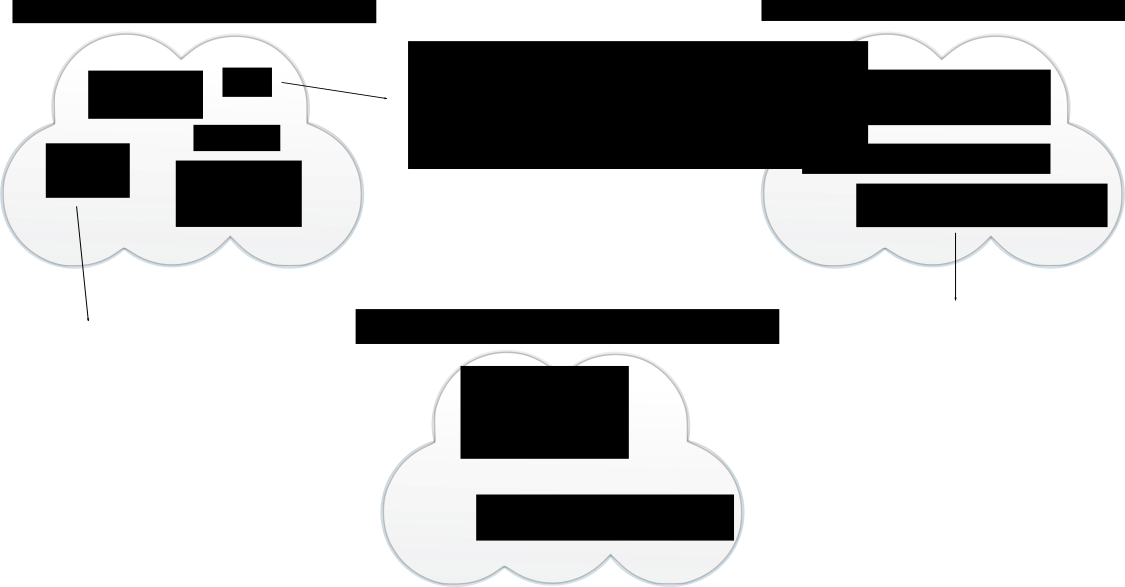
\includegraphics[width=\textwidth]{graphics/hmm-intro/time_series_problems_1_5.pdf}
  	\footnote{Sursa imaginii: http://desura.com}
  }
  \only<6>{
  	\includegraphics[width=\textwidth]{graphics/hmm-intro/time_series_problems_1_6.pdf}
  	\footnote{Sursa imaginii:  http://www.softpro.de}
  }
  
\end{frame}

\begin{frame}
  \frametitle{Probleme cu Secvențe Temporale (II)}
  \only<1>{
  	\includegraphics[width=\textwidth]{graphics/hmm-intro/time_series_problems_2.pdf}
  }
  \only<2>{
  	
\includegraphics[width=\textwidth]{graphics/hmm-intro/time_series_problems_2_2.pdf}
  	\footnote{Sursa imaginii:  http://www.econ.ucsb.edu/~doug/}
  }
\end{frame}


% descrierea a ceea ce inseamna Probabilistic Reasoning over Time (capitol 15.2 AI a modern approach)
% 	- states and observations
\begin{frame}[t]
  \frametitle{Raționament Probabilistic Temporal - Modele}
	
	Să ne gândim la unele din problemele anterioare ...	
	\vspace*{0.5em}
	\pause	
	
	Cum modelăm astfel de situații dinamice? 
	\vspace*{0.5em}
	\pause	
	
	\textbf{Stări și Observații}
	\begin{itemize}
		\item Procesul de schimbare este văzut ca o serie de \alert{snapshot-uri}
		\item Fiecare snapshot conține un set de variabile aleatoare
    	\begin{itemize}
			\item $\mathbf{O}_t$ - setul tuturor variabilelor de măsurare (\alert{\emph{observabile}}) la momentul \emph{t}
			\item $\mathbf{Q}_t$ - setul tuturor variabilelor de stare (\alert{\emph{neobservabile / ascunse}}) la momentul \emph{t}	    	
		\end{itemize}
	\end{itemize}
	
	\begin{figure}
		\centering
		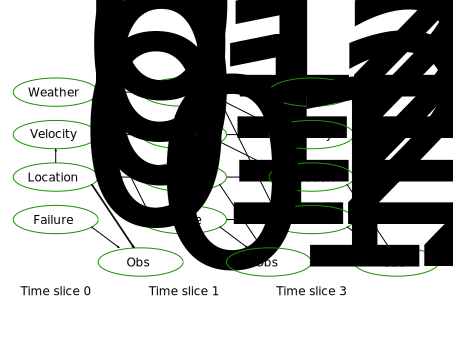
\includegraphics[height=0.3\textheight]{graphics/hmm-intro/dbn-vehicle/unrolled.pdf} 
  		\caption{\tiny{Exemplu: problemă de localizare a unui vehicul \citep{KollerFriedman09}}}
  		\label{fig:unrolled-states-observations}
  	\end{figure}
\end{frame}

%	- stationary process, Markov assumption, Sensor model
\begin{frame}[t]
  \frametitle{Raționament Probabilistic Temporal - Presupuneri}
	Să ne gândim la unele din problemele anterioare ...	
	\vspace*{0.5em}
	\pause	
	
	Ce \alert{presupuneri} (la o adică) facem?
	\pause	
	
	\begin{block}{Proces staționar}
		Procesul de schimbare este guvernat de legi care \alert{nu se schimba in timp}.\\
		\alert{Urmare:} trebuie sa specificăm relațiile între variabile doar pentru un snapshot \emph{reprezentativ}.	
	\end{block}
	\pause	
	
	\begin{block}{Presupunerea Markov}
		Starea curentă a unui proces de schimbare depinde doar de o \alert{istorie finită} de stări anterioare.\\
		\alert{Urmare:} avem un număr \alert{limitat} de ``parinți'' pentru variabilele din fiecare snapshot.
	\end{block}
  
\end{frame}

%	- inference in temporal models
%		- filtering
%		- prediction
%		- smoothing (hindsight)
%		- most likely explanation
%		- model learning
\begin{frame}
  \frametitle{Raționament Probabilistic Temporal - Inferență}
	Care sunt principalele inferențe ce se doresc făcute?	
	\pause	
	
	\begin{block}{Filtrare (monitorizare)}
		Sarcina de a calcula \alert{starea de fapt} - distribuția posterioară de probabilitate a 
		\alert{stării curente}, date fiind toate observațiile de până acum.
	\end{block}
	\pause
	
	\begin{block}{Evaluare}
		Sarcina de a calcula \alert{probabilitatea (likelihood)} a observațiilor făcute până în prezent.
	\end{block}  
\end{frame}

\begin{frame}
  \frametitle{Raționament Probabilistic Temporal - Inferență}
	\begin{block}{Predicție}
		Sarcina de a calcula distribuția posterioară de probabilitate peste o \alert{stare viitoare}, 
		date fiind toate observațiile de până acum.
	\end{block}
	\pause
	
	\begin{block}{Netezire (hindsight)}
		Sarcina de a calcula distribuția posterioară de probabilitate peste o \alert{stare anterioară}, 
		date fiind toate observațiile de până acum.\\
		Furnizează o estimare mai buna asupra stării respective, decât a fost posibil la momentul respectiv.
	\end{block}
\end{frame}

\begin{frame}
  \frametitle{Raționament Probabilistic Temporal - Inferență}
	\begin{block}{Cea mai probabilă explicație}
		Dându-se o \emph{secvență de observații}, se cere găsirea \alert{celei mai probabile secvenței de stări}
		care a generat acele observații.
	\end{block}
	\pause
	
	\begin{block}{Învățare}
		Dându-se \emph{un set de secvențe de observații}, găsește o metodă de a învăța \alert{modelele} de
		\alert{tranziție} și \alert{senzoriale / de măsurare} pe baza acelor observații.
	\end{block}
\end{frame}

\begin{frame}[t]
    \frametitle{Raționament Probabilistic Temporal - Metode Cunoscute}
    
  	\begin{block}{Rețele Bayesiene Dinamice (RBD)}
  		O RBD este o rețea Bayesiană ce reprezintă un model temporal de probabilitate.
  	\end{block}
  	
  	\begin{figure}
  		\centering
		\begin{subfigure}[b]{0.15\textwidth}
			\centering
  			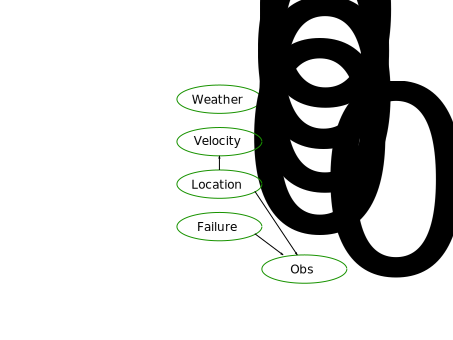
\includegraphics[width=\textwidth]{graphics/hmm-intro/dbn-vehicle/zero.pdf}
  			\caption{\tiny{Rețeaua Bayesiană în două snapshot-uri}}
  			\label{fig:2TBN}
  		\end{subfigure}
  		\begin{subfigure}[b]{0.30\textwidth}
			\centering
			\includegraphics[width=\textwidth]{graphics/hmm-intro/dbn-vehicle/transition.pdf}
  			\caption{\tiny{Rețeaua la momentul 0}}
  			\label{fig:zeroDBN}
  		\end{subfigure}
  		\begin{subfigure}[b]{0.35\textwidth}
			\centering
			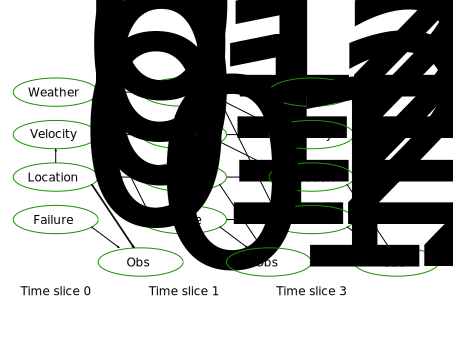
\includegraphics[width=\textwidth]{graphics/hmm-intro/dbn-vehicle/unrolled.pdf} 
  			\caption{\tiny{RBD desfășurată pe 3 momente de timp}}
  			\label{fig:unrolledDBN}
  		\end{subfigure}
  		\caption{\tiny{RBD simplificată pentru monitorizarea unui vehicul \citep{KollerFriedman09}}}
  		\label{fig:DBN}
  	\end{figure}
  	
  	\small{Aplicată în probleme precum: urmărirea obiectelor, recunoașterea activității umane, secvențierea proteinelor, etc.}
\end{frame}


\begin{frame}[t]
    \frametitle{Raționament Probabilistic Temporal - Metode Cunoscute}
  
  \begin{block}{Filtre Kalman (Sistem Dinamice Lineare)}
	Un model temporal având una sau mai multe variabile care evoluează linear în timp, la care se adaugă 
	\alert{zgomot Gaussian}.
  \end{block}
  
  \begin{columns}[T]
  	\column{0.4\textwidth}
  	\begin{figure}
  		\centering
  		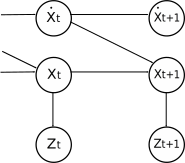
\includegraphics[height=0.35\textheight]{graphics/hmm-intro/kalman/kalman_filter_simple.pdf}
  		\caption{\tiny{Structura unei RB pentru un sistem linear dinamic cu variabile de poziție $X_t$, 
  		viteză $\dot{X}_t$, și măsurare a poziției $Z_t$}}
  	\end{figure}
	  
  	\column{0.6\textwidth}
  	\begin{itemize}
  		\item \footnotesize{Poate fi văzut ca o RBD în care toate variabilele sunt continue, iar dependențele sunt 
  		linear gaussiane.}
  		\item \footnotesize{Aplicații multiple în \textbf{urmărirea obiectelor}}
  	\end{itemize}
  \end{columns}
  
\end{frame}

\begin{frame}[t]
    \frametitle{Raționament Probabilistic Temporal - Metode Cunoscute}
  
  \begin{block}{Modele Markov Ascunse (MMA)}
	Un MMA (HMM) este un model probabilistic temporal în care \emph{starea} procesului de schimbare este descrisă
	de \alert{o singură variabilă aleatoare discretă}.
	Valorile posibile ale variabilei reprezintă stările posibile ale lumii modelate.
  \end{block}
  
  \vspace*{1em}
  
  Utilizat cu succes in aplicații precum:
  \begin{itemize}
  	\item Recunoasțerea Scrisului
  	\item Recunoasțerea Gesturilor
  	\item Recunoasțerea Vorbirii
  	\item Determinarea Parților de Vorbire (Part-of-Speech Tagging)
  	\item Secvențiere ADN
  \end{itemize}
\end{frame}



\section{Teoria MMA}
\label{sec:theory}

\subsection{Cele Trei Probleme ale MMA}
\label{sec:three-problmes}

%% alejandro
\section{Theory of HMMs}
\label{sec:theory}

\subsection{The 3 things you want from an HMM}
\label{sec:problems}

\begin{frame}
  
  The 3 fundamental problems \parencite{rabiner1989tutorial}
  \begin{itemize}
  	\item Particularization of temporal inference problems to the HMM case
  	\item The restricted structure of the HMM allows for elegant implementations of all the basic algorithms
  \end{itemize}
  \pause

  \begin{block}{Evaluation Problem}
    Given a model and a sequence of observations, how do we compute the probability that the \alert{observed 
    sequence} was produced by the model?
  \end{block}
  \pause
  \begin{block}{Best Explanation of Observations Problem}
    Given a model and a sequence of observations how do we choose a corresponding sequence of \alert{states} which 
    \emph{gives meaning} to the observations? How do we \emph{uncover} the hidden part of the model?
  \end{block}
  \pause
  \begin{block}{Model Estimation (Training) Problem}
    Given some observed sequences, how do we adjust the \alert{parameters} of an HMM model that best tries to explain 
    the observations? 
    
  \end{block}

\end{frame}


\subsection{Mathematical Foundations for HMMs}
\label{sec:math}


\begin{frame}
  \frametitle{An example problem: Emotional states}
  \begin{columns}[T]
    \column{0.58\textwidth}
    \only<1>{\framebox{\includegraphics[width=\textwidth]{graphics/example/hmm-final-m.pdf}}}
    \only<2>{\framebox{\includegraphics[width=\textwidth]{graphics/example/hmm-final-n.pdf}}}
    \only<3>{\framebox{\includegraphics[width=\textwidth]{graphics/example/hmm-final-o.pdf}}}
    \only<4>{\framebox{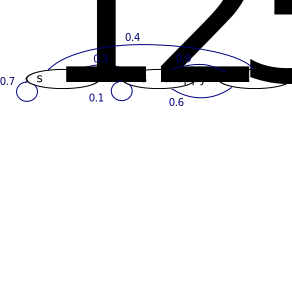
\includegraphics[width=\textwidth]{graphics/example/hmm-final-q.pdf}}}
    \only<5>{\framebox{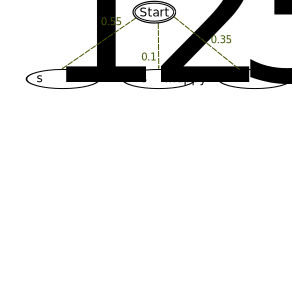
\includegraphics[width=\textwidth]{graphics/example/hmm-final-r.pdf}}}
    \only<6>{\framebox{\includegraphics[width=\textwidth]{graphics/example/hmm-final-s.pdf}}}
    \only<7>{\framebox{\includegraphics[width=\textwidth]{graphics/example/hmm-final-t.pdf}}}
    \only<8>{\framebox{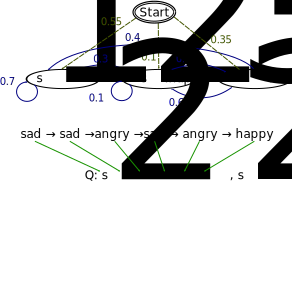
\includegraphics[width=\textwidth]{graphics/example/hmm-final-u.pdf}}}
    \only<9>{\framebox{\includegraphics[width=\textwidth]{graphics/example/hmm-final-v.pdf}}}
    \only<10>{\framebox{\includegraphics[width=\textwidth]{graphics/example/hmm-final-v2.pdf}}}
    \only<11-12>{\framebox{\includegraphics[width=\textwidth]{graphics/example/hmm-final-w.pdf}}}
    \only<13>{\framebox{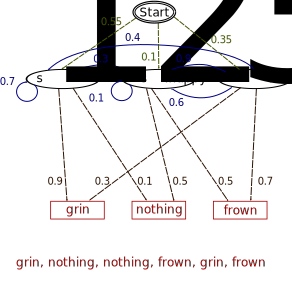
\includegraphics[width=\textwidth]{graphics/example/hmm-final-x.pdf}}}
    \only<14>{\framebox{\includegraphics[width=\textwidth]{graphics/example/hmm-final-y.pdf}}}
    \only<15>{\framebox{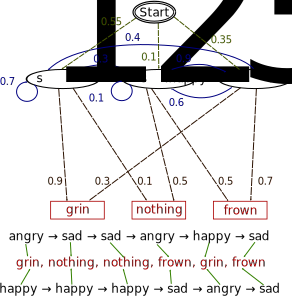
\includegraphics[width=\textwidth]{graphics/example/hmm-final-z.pdf}}}
    \only<16> {
      \begin{itemize}
      \item Example inspired from: \\\vspace*{1em}
        \fullcite{zubek2006introduction}
      \end{itemize}

    }
    

    \column{0.4\textwidth} \only<1>{ Let's consider a simple example:
      \\ \ a robot that tracks the emotional states of a player.  }
    \only<2>{ $\mathbf{N}$ - number of states \\ \vspace*{.5em}
      $\mathbf{N}=3$ \\ \vspace*{.5em} states:
      \begin{itemize}
      \item $s_1$: happy
      \item $s_2$: sad
      \item $s_3$: angry
      \end{itemize}

    }\only<3-4> { $\mathbf{A}$ - state transition probability
      distribution \\ \vspace*{.5em} \small{ $\mathbf{A} = \lbrace
        a_{i,j} \rbrace, \: 1 \le i, j \le N$ \\ \vspace*{.5em}
        $a_{i,j} = P(q_{t+1}=s_j \vert q_t = s_i)$
        \begin{itemize}
        \item $a_{\mathbf{1},1} = 0.7$
        \item $a_{\mathbf{1},2} = 0.3$
        \item $a_{\mathbf{1},3} = 0$
        \end{itemize}
        $\displaystyle\sum_{j=1}^{N}a_{i,j}=1, \quad 1 \le i \le N$ }
      \visible<4-> { $\mathbf{A} = \bordermatrix{~ & s_1 & s_2 & s_3
          \cr s_1 & 0.7 & 0.3 & 0 \cr s_2 & 0 & 0.9 & 0.1 \cr s_3 &
          0.4 & 0.6 & 0 \cr}$ }

    }
    
    \only<5>{ $\mathbf{\Pi}$ - initial state distribution \\
      \vspace*{0.5em} $\mathbf{\Pi} = \lbrace \pi_i \rbrace,\quad 1
      \le i \le N$ \\ \vspace*{0.5em} $\pi_i = P(q_1 = s_i)$ \\
      \vspace*{0.5em}
      
      $ \mathbf{\Pi} = \bordermatrix{ ~ & s_1 & s_2 & s_3 \cr ~ & 0.35
        & 0.1 & 0.55 \cr} $ }
    
    \only<6-8>{ $A = \bordermatrix{~ & s_1 & s_2 & s_3 \cr s_1 & 0.7 &
        0.3 & 0 \cr s_2 & 0 & 0.9 & 0.1 \cr s_3 & 0.4 & 0.6 & 0 \cr}$
      \\ \vspace*{0.25em} $\Pi = \bordermatrix{ ~ & s_1 & s_2 & s_3
        \cr ~ & 0.35 & 0.1 & 0.55 \cr}$ \\ \vspace*{0.25em}
      \visible<8> { $Q = [ q_1 q_2 \cdots q_T ]$ \small{
          \begin{equation*}
            \begin{split}
              P(Q & \vert A,\Pi)= \\ & = \pi_{q_1}a_{q_1,q_2}\cdots
              a_{q_{T-1},q_T}
            \end{split}
          \end{equation*}
          \begin{equation*}
            \begin{split}
              P(s_2,s_2,s_3,s_2,s_3,s_1\vert A,\Pi) = \\
              = \pi_2 \cdot a_{2,2} \cdot a_{2,3} \cdot a_{3,2} \cdot a_{2,3} \cdot a_{3,1} \\
              = \scriptstyle{0.1 \cdot 0.3 \cdot 0.1 \cdot 0.9 \cdot 0.6 \cdot 0.9 \cdot 0.4} \\
              = \scriptstyle{0.0005832}
            \end{split}
          \end{equation*}
        } }}

    \only<9>{ $\mathbf{M}$ - number of distinct observable values \\
      \vspace*{.5em} $\mathbf{M}=3$ \\ \vspace*{.5em} values:
      \begin{itemize}
      \item $v_1$: grin
      \item $v_2$: nothing
      \item $v_3$: frown
      \end{itemize}
    }

    \only<10-11> { $\mathbf{B}$ - observation values probability
      distribution \\ \vspace*{.5em} \small{ $\mathbf{B} = \lbrace
        b_{j,k} \rbrace \: \scriptstyle{1 \le j \le N, 1 \le k, \le
          M}$
        \begin{equation*}
          \begin{split}
            b_{j,k} & =b_{j}(v_k) \\
            & =P(o_t = v_k \vert q_t = s_j)
          \end{split}
        \end{equation*}
        \vspace*{-1.5em} \scriptsize{
          \begin{itemize}
          \item $b_{\mathbf{1},1} = b_{\mathbf{1}}(grin) = 0.9$
          \item $b_{\mathbf{1},2} = b_{\mathbf{1}}(nothing) = 0.1$
          \item $b_{\mathbf{1},3} = b_{\mathbf{1}}(frown) = 0$
          \end{itemize}}
        $\displaystyle\sum_{k=1}^{M}b_{j,k}=1, \quad 1 \le j \le N$\\
      }\visible<11> { $\mathbf{B} = \bordermatrix{ ~ & grin & notg &
          frown \cr s_1 & 0.9 & 0.1 & 0 \cr s_2 & 0 & 0.5 & 0.5 \cr
          s_3 & 0.3 & 0 & 0.7 \cr }$ } }
    
    \only<12>{ $\mathbf{\lambda}$ - parameters of the model \\
      \vspace*{.5em} $\lambda = (A, B, \Pi)$ \\ \vspace*{2em} $A$ -
      state transition probability distribution \\ \vspace*{.5em} $B$
      - observation values probability distribution \\ \vspace*{.5em}
      $\Pi$ - initial state distribution }
    
    \only<13-15>{ $\mathbf{O}$ - observation sequence \\ \vspace*{1em}
      $\mathbf{T}$ - length of observation sequence \\ \vspace*{1em}
      $O = [ o_1 o_2 \cdots o_T ]$ }

  \end{columns}
\end{frame}

\begin{frame}[T]
  \frametitle{Restating the three fundamental HMM Problems}
  
  \begin{block}{Evaluation Problem}
    Given a model \visible<2->{\alert{$\lambda=(A,B,\Pi)$}} and a
    sequence of observations \visible<3->{\alert{$O = [ o_1 o_2 \cdots
        o_T ]$}}, how do we compute the probability
    \visible<4->{\alert{$P(O \vert \lambda)$}} that the
    observed sequence was produced by the model? \\
  \end{block}
  \visible<5->{
  
    \begin{itemize}
    \item Enumerate every possible state sequence:

      \begin{equation}
        \begin{split}
          P(O \vert \lambda) = \displaystyle\sum_{\text{all}\;Q} P(O
          \vert Q, \lambda) \cdot P(Q \vert \lambda)
        \end{split}
        \label{eq1}
      \end{equation}
    \end{itemize}
    
  }
\end{frame}

\begin{frame}
  \frametitle{Restating the three fundamental HMM Problems}
  \begin{equation}
    \begin{split}
      P(O \vert \lambda) = \displaystyle\sum_{\text{all}\;Q} P(O \vert
      Q, \lambda) \cdot P(Q \vert \lambda)
    \end{split}
    \tag{\ref{eq1}}
  \end{equation}
  \pause \vspace*{.em}
  \begin{equation}
    P(O \vert Q, \lambda) = \displaystyle\prod_{t=1}^{T} P(o_t \vert
    q_t, \lambda)= \displaystyle\prod_{t=1}^{T} b_{q_t}(o_t) =
    b_{q_1}(o_1) \cdot \ldots \cdot b_{q_T}(o_T)
    \label{eq:pql}
  \end{equation}\pause
  \vspace*{.em}
  \begin{equation}
    P(Q | \lambda) = \pi_{q_1}\displaystyle\prod_{t=2}^{T}
    a_{q_{t-1},q_t} = \pi_{q_1} \cdot a_{q_1,q_2} \cdot a_{q_2,q_3} \cdot \ldots \cdot
    a_{q_{T-1},q_T}\label{eq:pql2}
  \end{equation}\pause
  \vspace*{.em}
  \begin{equation}
    \begin{split}
      P(O \vert \lambda) = \displaystyle\sum_{all\;Q} P(O, Q \vert
      \lambda) & = \displaystyle\sum_{all\;Q} P(O,\vert Q, \lambda)
      \cdot P(Q, \lambda) \\
      & = \displaystyle\sum_{\text{all}\;Q} \Big( \pi_{q_1} \cdot
      b_{q_1}(o_1) \cdot \displaystyle\prod_{t=2}^{T} b_{q_t}(o_t)
      a_{q_{t-1},q_t} \Big)
    \end{split}
    \tag{\ref{eq1}}
  \end{equation}
\end{frame}

\begin{frame}
  \frametitle{Restating the three fundamental HMM Problems}
  \begin{block}{Best Explanation of Observations Problem}
    Given a model \visible<2->{\alert{$\lambda=(A,B,\Pi)$}} and a
    sequence of observations \visible<3->{\alert{$O = [ o_1 o_2 \cdots
        o_T ]$}} how do we choose a corresponding sequence of
    \alert{states} \visible<4->{\alert{$Q = [ q_1 q_2 \cdots q_T ]$}}
    which \emph{gives meaning} to the observations?  How do we
    \emph{uncover} the hidden part of the model?
  \end{block}
  \visible<5->{
    \begin{itemize}
    \item There is no single answer.
    \item The sequence of individually most likely states:
      \begin{equation}
        \label{eq:inidi}
        Q_{\text{best}} = [\hat{q}_1\; \hat{q}_2\; \ldots \hat{q}_T], 
        \quad \hat{q}_t = \underset{s_i}{argmax}\; P(q_t = s_i \vert O, \lambda)
      \end{equation}
      
    \visible<6->{\item The best path
      \begin{equation}
        Q_{\text{best}} = \underset{Q}{\operatorname{argmax}}\;
        P(Q \vert O, \lambda)
        = \underset{Q}{\operatorname{argmax}}\; P(Q, O \vert \lambda)
        \label{eq:best-explanation}
      \end{equation}}
    \end{itemize}
  }
\end{frame}




\begin{frame}
  \frametitle{Restating the three fundamental HMM Problems}
  \begin{block}{Model Estimation (Training) Problem}
    Given some observed sequences \visible<2->{\alert{$\mathcal{O} =
        [O_1 O_2 \cdots O_L]$}}, how do we adjust the
    \alert{parameters} \visible<3->{\alert{$\lambda=(A,B,\Pi)$}} of an
    HMM model that best tries to explain the observations?
  \end{block}
  \visible<4->{
    \begin{itemize}
    \item The above question can be asked formally:
      \begin{equation}
        \lambda_{\text{best}} = \underset{\lambda}{\operatorname{argmax}}\;
        P(\mathcal{O} \vert \lambda)
        \label{eq:best-explanation}
      \end{equation}
    \end{itemize}
  }
\end{frame}



\subsection{Notation Conventions \& Framework Description}
\label{sec:octave}

\begin{frame}
  \frametitle{Notation Conventions}

  
\end{frame}


\begin{frame}
  \frametitle{Variables in Octave}

  
\end{frame}


\subsection{Fundamente Matematice}
\label{sec:math-foundations}

%% tudor
%% Tudor Berariu, Alexandru Sorici
%% Noiembrie 2012

%% În această secțiune vom descrie din punct de vedere matematic
%% modelele Markov ascunse și vom reformula cele trei probleme
%% fundamentale în termeni de probabilități.

%%%%%%%%%%%%%%%%%%%%%%
%% Slide 0: Intro
\begin{frame}
  \frametitle{O perspectivă teoretică asupra MMA}
  \begin{itemize}
  \item Vom răspunde la următoarele întrebări:
    \begin{enumerate}
      \vspace*{1em}
    \item Cum definim un Model Markov Ascuns?
      \vspace*{1em}
    \item Cum exprimăm cele trei întrebări fundamentale cu ajutorul probabilităților?
    \end{enumerate}
  \end{itemize}
\end{frame}

%%%%%%%%%%%%%%%%%%%%%%
%% Slide 1: Definiție
%% În teoria semnalelor, MMA descriu situații în care un sistem stocastic 
%% este observat prin măsurători afectate de zgomot.
\begin{frame}
  \frametitle{Ce este un MMA?}
  \begin{block}{Definiție}
    Un \alert{Model Markov Ascuns} este un dublu proces stocastic cu două componente:
    \begin{itemize}
    \item un proces Markov \visible<2>{\emph{neobservabil} (\emph{ascuns}),
    \item un set de procese stocastice care produc partea \emph{observabilă}.}
    \end{itemize}
  \end{block}
  \vspace*{1em}
  \framebox{%
    \only<1>{%
      \includegraphics[width=\textwidth]{graphics/definition/mp-sequence.pdf}
    }%
    \only<2>{%
      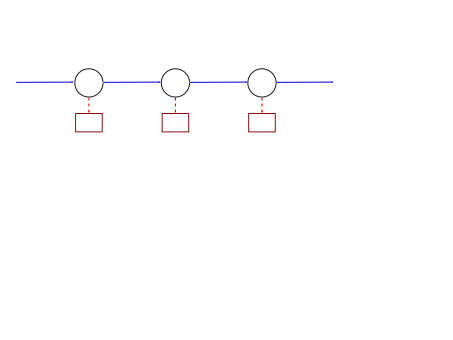
\includegraphics[width=\textwidth]{graphics/definition/hmm-sequence.pdf}
    }%
  }
\end{frame}


%%%%%%%%%%%%%%%%%%%%%%

%%%%%%%%%%%%%%%%%%%%%%
%% Slide 2: Construim un exemplu
\begin{frame}
  \frametitle{Exemplu: Urmărirea stărilor emoționale}
  \begin{columns}[T]
    \column{0.58\textwidth}
    \only<1>{\framebox{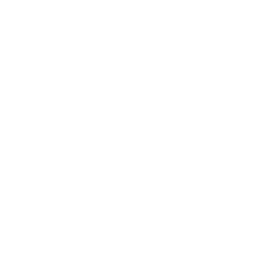
\includegraphics[width=\textwidth]{graphics/toy-example/example-k.pdf}}}%
    \only<2>{\framebox{\includegraphics[width=\textwidth]{graphics/toy-example/example-l.pdf}}}%
    \only<3>{\framebox{\includegraphics[width=\textwidth]{graphics/toy-example/example-m.pdf}}}%
    \only<4>{\framebox{\includegraphics[width=\textwidth]{graphics/toy-example/example-n.pdf}}}%
    \only<5>{\framebox{\includegraphics[width=\textwidth]{graphics/toy-example/example-o.pdf}}}%
    \only<6>{\framebox{\includegraphics[width=\textwidth]{graphics/toy-example/example-p.pdf}}}%
    \only<7>{\framebox{\includegraphics[width=\textwidth]{graphics/toy-example/example-q.pdf}}}%
    \only<8>{\framebox{\includegraphics[width=\textwidth]{graphics/toy-example/example-r.pdf}}}%
    \only<9>{\framebox{\includegraphics[width=\textwidth]{graphics/toy-example/example-s.pdf}}}%
    \only<10>{\framebox{\includegraphics[width=\textwidth]{graphics/toy-example/example-t.pdf}}}%
    \only<11>{\framebox{\includegraphics[width=\textwidth]{graphics/toy-example/example-t2.pdf}}}%
    \only<12>{\framebox{\includegraphics[width=\textwidth]{graphics/toy-example/example-u.pdf}}}%
    \only<13>{\framebox{\includegraphics[width=\textwidth]{graphics/toy-example/example-v.pdf}}}%
    \only<14>{\framebox{\includegraphics[width=\textwidth]{graphics/toy-example/example-w.pdf}}}%
    \only<15>{\framebox{\includegraphics[width=\textwidth]{graphics/toy-example/example-x.pdf}}}%
    \only<16>{\framebox{\includegraphics[width=\textwidth]{graphics/toy-example/example-y.pdf}}}%
    \only<17>{\framebox{\includegraphics[width=\textwidth]{graphics/toy-example/example-z.pdf}}}%
    \column{0.4\textwidth}%
    \only<1>{%
      Să considerăm următorul exmeplu:
      \begin{itemize}
      \item un robot ce urmărește evoluția stărilor emoționale ale
        unui om
      \end{itemize}
      \vspace*{1em} Senzor:
      \begin{itemize}
      \item cameră video
      \end{itemize}
      \vspace*{1em}
      Exemplu adaptat după :\\\vspace*{.5em}
      \def\newblock{}\nobibliography{}\bibentry{zubek2006introduction}
    }\only<2>{%
      $\mathbf{N}$ - numărul de stări ascunse\\%
      $\mathbf{S}$ - mulțimea stărilor\\\vspace*{.5em}%
      \horiline%
      $\mathbf{N}=3$ \\\vspace*{.5em}%
      Stări:
      \begin{itemize}
      \item $\mathbf{s_1}$: vesel
      \item $\mathbf{s_2}$: trist
      \item $\mathbf{s_3}$: nervos
      \end{itemize}
    }\only<3-5>{%
      $\mathbf{A}$ - matricea distribuțiilor de
      probabilitate ale tranzițiilor între stări\\\vspace*{.5em}%
      \small{%
        $\mathbf{A} = \lbrace a_{i,j} \rbrace, \: 1 \le i, j \le N$\\\vspace*{.5em}%
        $a_{i,j} = P(q_{t+1}=s_j \vert q_t = s_i)$\\%
        \horiline%
        $\displaystyle\sum_{j=1}^{N}a_{i,j}=1, \quad 1 \le i \le N$}\\%
      \horiline%
      \visible<3->{%
        $\mathbf{A} = \bordermatrix{~ & s_1 &
          s_2 & s_3 \cr s_1 & 0.8 & 0.1 & 0.1 \cr s_2 &
          \visible<4->{0.25} & \visible<4->{0.25} & \visible<4->{0.5}
          \cr s_3 & \visible<5->{0.8} & \visible<5->{0.2} &
          \visible<5->{0} \cr}$ }%
    }\only<6>{%
      $\mathbf{\Pi}$ - distribuția stării inițiale\\\vspace*{0.5em}%
      $\mathbf{\Pi} = \lbrace \pi_i \rbrace,\quad 1 \le i \le N$\\\vspace*{0.5em}%
      $\pi_i = P(q_1 = s_i)$\\\vspace*{0.5em}%
      $\mathbf{\Pi} = \bordermatrix{ ~ & s_1 & s_2 & s_3 \cr ~ & 0.7 & 0.2 & 0.1 \cr}$%
    }\only<7-8>{%
      Deocamdată am descris un \emph{proces Markov}.\\\vspace*{0.25em}%
      $A = \bordermatrix{~ & s_1 & s_2 & s_3 \cr s_1 & 0.8 & 0.1 & 0.1 \cr s_2
        & 0.25 & 0.25 & 0.5 \cr s_3 & 0.8 & 0.2 & 0 \cr}$\\\vspace*{0.25em}%
      $\Pi = \bordermatrix{ ~ & s_1 & s_2 & s_3 \cr ~ & 0.7 & 0.2 & 0.1 \cr}$\\%
      \horiline%
      \visible<8>{%
        Notație: $\mathbf{Q} = [ q_1 q_2 \cdots q_T ]$%
        \horiline%
        \begin{equation*}
          \begin{array}{l}
            \scriptstyle
              P(Q \vert A,\Pi) = \pi_{q_1}a_{q_1,q_2}\cdots a_{q_{T-1},q_T} \\
              \scriptstyle
              P(s_1,s_1,s_3,s_2\vert A,\Pi) = \pi_1 \cdot a_{1,1} \cdot a_{1,3} \cdot a_{3,2}= \\
              \scriptstyle
              = 0.8\; \cdot\; 0.8\; \cdot\; 0.1\; \cdot\; 0.2 = 0.0128
          \end{array}%
        \end{equation*}%
      }}\only<9>{%
      $\mathbf{M}$ - numărul de valori observabile distincte\\\vspace*{.5em}%
      $\mathbf{M}=3$\\\vspace*{.5em}
      valori observabile:
      \begin{itemize}
      \item $\mathbf{v_1}$: zâmbmet / rânjet
      \item $\mathbf{v_2}$: nimic
      \item $\mathbf{v_3}$: încruntare
      \end{itemize}%
    }\only<10-12>{%
      $\mathbf{B}$ - matricea distribuțiilor de probabilitate ale valorilor
      observabile\\\vspace*{.5em}
      \small{% 
        $\mathbf{B} = \lbrace b_{j,k} \rbrace \: \scriptstyle{1
          \le j \le N, 1 \le k, \le M}$
        \begin{equation*}
          \begin{split}
            b_{j,k} & =b_{j}(v_k) \\
            & =P(o_t = v_k \vert q_t = s_j)
          \end{split}
        \end{equation*}%
        \vspace*{-.5em}\horiline%
        $\displaystyle\sum_{k=1}^{M}b_{j,k}=1, \quad 1 \le j \le N$%
      }%
      \horiline%
      \visible<10->{ $\mathbf{B} = \bordermatrix{~ & v_1 &
          v_2 & v_3 \cr s_1 & 0.7 & 0.3 & 0 \cr s_2 &
          \visible<11->{0} & \visible<11->{0.7} & \visible<11->{0.3}
          \cr s_3 & \visible<12->{0.6} & \visible<12->{0} &
          \visible<12->{0.4} \cr}$}%
    }\only<13>{% 
      $\mathbf{\lambda}$ - parametrii Modelului Markov Ascuns\\\vspace*{.5em}%
      $\lambda = (A, B, \Pi)$\\\vspace*{2em}%
      $A$ - matricea distribuțiilor de probabilitate ale tranzițiilor între
      stări\\\vspace*{.5em}%
      $B$ - matricea distribuțiilor de probabilitate ale valorilor observabile\\\vspace*{.5em}%
      $\Pi$ - distribuția stării inițiale%
    }\only<14-17>{%
      $\mathbf{O}$ - secvența de observații\\\vspace*{1em}%
      $\mathbf{T}$ - lungimea secvenței de observații\\\vspace*{1em}%
      $O = [ o_1 o_2 \cdots o_T ]$% 
    }%
  \end{columns}
\end{frame}
%%%%%%%%%%%%%%%%%%%%%%

%%%%%%%%%%%%%%%%%%%%%%
%% Slide 3: Din ce este compus un HMM
\begin{frame}
  \frametitle{Modele Markov Ascunse}
  \begin{block}{Definiție}
    Un \alert{Model Markov Ascuns} este un tuplu $\langle S,V,A,B,P \rangle$:
    \begin{itemize}
    \item $S$ - mulțimea stărilor
    \item $V$ - mulțimea valorilor observabile
    \item $A$ - matricea de tranziție
    \item $B$ - matricea de emisie
    \item $\Pi$ - matricea distribuției stării inițiale
    \end{itemize}
  \end{block}
  \begin{itemize}
  \item Notație: $\lambda=(A,B,\Pi)$ - parametrii modelului
  \end{itemize}
  \vspace*{.5em}
  \begin{center}%
    \framebox{%
      \includegraphics[width=.6\textwidth]{graphics/definition/hmm-sequence-adnotated.pdf}%
    }%
  \end{center}
\end{frame}
%%%%%%%%%%%%%%%%%%%%%% 


%%%%%%%%%%%%%%%%%%%%%%
%% Slide 4: Problema evaluării

\begin{frame}[T]
  \frametitle{Reformularea problemelor fundamentale ale MMA}
  \begin{block}{Problema evaluării}
    Date fiind un model \visible<2->{\alert{$\lambda=(A,B,\Pi)$}} și o
    secvență de observații \visible<2->{\alert{$O = [ o_1 o_2 \cdots
        o_T ]$}}, cum calculăm probabilitatea \visible<2->{\alert{$P(O
        \vert \lambda)$}} ca secvența de observații să fi fost
    generată de acel model?
  \end{block}
  \visible<3->{%
    \begin{itemize}
    \item Prin enumerarea tuturor secvențelor posibile de stări:
      \begin{equation}
          P(O \vert \lambda) = \displaystyle\sum_{\text{all}\;Q} P(O
          \vert Q, \lambda) \cdot P(Q \vert \lambda)
        \label{eq1}
      \end{equation}
      (legea probabilității totale)
    \end{itemize}
  }
\end{frame}

%%%%%%%%%%%%%%%%%%%%%%
%% Slide 5: Prelucrarea formulei

\begin{frame}[t]
  \frametitle{Reformularea problemelor fundamentale ale MMA}
  \vspace*{-1em}%
  \begin{equation}
      P(O \vert \lambda) = \displaystyle\sum_{\text{all}\;Q} P(O \vert
      Q, \lambda) \cdot P(Q \vert \lambda)
    \tag{\ref{eq1}}
  \end{equation}%
  \horiline%
  \visible<2->{%
    \small{Primul factor (independență condițională):}
    \begin{equation}
      P(O \vert Q, \lambda) = \displaystyle\prod_{t=1}^{T} P(o_t \vert
      q_t, \lambda)= \displaystyle\prod_{t=1}^{T} b_{q_t}(o_t) =
      b_{q_1}(o_1) \cdot \ldots \cdot b_{q_T}(o_T)
      \label{eq:pql}
    \end{equation}%
    \visible<3->{%
      \small{Al doilea factor (presupunerea Markov):}
      \begin{equation}
        P(Q | \lambda) = \pi_{q_1}\displaystyle\prod_{t=2}^{T}
        a_{q_{t-1},q_t} = \pi_{q_1} \cdot a_{q_1,q_2} \cdot a_{q_2,q_3} \cdot \ldots \cdot
        a_{q_{T-1},q_T}\label{eq:pql2}
      \end{equation}%
      \horiline%
      \visible<4->{%
        \begin{equation}
          P(O \vert \lambda)  = \displaystyle\sum_{\text{all}\;Q} \Big( \pi_{q_1} \cdot
            b_{q_1}(o_1) \cdot \displaystyle\prod_{t=2}^{T} b_{q_t}(o_t)
            a_{q_{t-1},q_t} \Big)
          \tag{\ref{eq1}}
        \end{equation}
      }%
    }%
  }%
\end{frame}
%%%%%%%%%%%%%%%%%%%%%%

%%%%%%%%%%%%%%%%%%%%%%
%% Slide 6: Problema 2
\begin{frame}
  \frametitle{Reformularea problemelor fundamentale ale MMA}
  \begin{block}{Problema interpretării unei secvențe de observații}
    Date fiind un model \visible<2->{\alert{$\lambda=(A,B,\Pi)$}} și o
    secvență de observații \visible<3->{\alert{$O = [ o_1 o_2 \cdots
        o_T ]$}}, cum alegem o secvență corespunzătoare de stări
    \visible<4->{\alert{$Q = [ q_1 q_2 \cdots q_T ]$}} care \emph{să
      dea un înțeles} observațiilor? Cum \emph{descoperim} partea
    ascunsă a modelului?
  \end{block}
  \visible<5->{%
    \begin{itemize}
    \item Există mai multe criterii pentru \emph{cea mai bună} sevență
      \begin{itemize}
      \item Secvența celor mai probabile stări (luate individual):
        \begin{equation}
          \label{eq:inidi}
          Q_{\text{best}} = [\hat{q}_1\; \hat{q}_2\; \ldots \hat{q}_T], 
          \quad \hat{q}_t = \underset{s_i}{argmax}\; P(q_t = s_i \vert O, \lambda)
        \end{equation}%
        \visible<6->{\item Cea mai bună $cale$ (de dimensiune $T$)
          \begin{equation}
            Q_{\text{best}} = \underset{Q}{\operatorname{argmax}}\;
            P(Q \vert O, \lambda)
            = \underset{Q}{\operatorname{argmax}}\; P(Q, O \vert \lambda)
            \label{eq:best-explanation}
          \end{equation}}
      \end{itemize}
    \end{itemize}
  }%
\end{frame}

%%%%%%%%%%%%%%%%%%%%%%
%% Slide 7: Problema 3

\begin{frame}
  \frametitle{Reformularea problemelor fundamentale ale MMA}
  \begin{block}{Problema Estimării Modelului (Învățării)}
    Date fiind niște secvențe de observații
    \visible<2->{\alert{$\mathcal{O} = [O_1 O_2 \cdots O_L]$}}, cum
    \emph{ajustăm} \alert{parametrii}
    \visible<3->{\alert{$\lambda=(A,B,\Pi)$}} ai unui MMA astfel încât
    să explice cel mai bine observațiile?
  \end{block}
  \visible<4->{
    \begin{itemize}
    \item Întrebarea se poate reformula matematic:
      \begin{equation}
        \lambda_{\text{best}} = \underset{\lambda}{\operatorname{argmax}}\;
        P(\mathcal{O} \vert \lambda)
        \label{eq:best-explanation}
      \end{equation}
    \end{itemize}
  }
\end{frame}
%%%%%%%%%%%%%%%%%%%%%%


\subsection*{Descrierea Platformei de Lucru}
\label{sec:framework}

%% tudor
\begin{frame}
  \frametitle{Mediul de lucru}
Pentru început
  \begin{enumerate}
  \item Deschideți \texttt{Matlab} / \texttt{Octave}
  \item Schimbați directorul de lucru cu \texttt{aria-hmm}
  \item Adăugați toate subdirectoarele în path:\\
    \mcode{addpath(genpath('.'))}
  \end{enumerate}
\end{frame}

\begin{frame}
  \frametitle{Platforma de lucru - fișierele stub}
  Fișierele \texttt{.stub}
  \begin{itemize}
  \item le veți folosi ca schelet de cod pentru sesiunile de implementare
  \item au sectiuni delimitate de \texttt{<label>-start} și \texttt{<label>-end}
    între care veți adăuga liniile de cod
  \item înlăturați sufixul \texttt{.stub} când rezolvați task-urile.
  \end{itemize}\vspace*{-1em}%
  \lstinputlisting{m-files/forward-backward.m}
\end{frame}

\begin{frame}
  \frametitle{Platforma de lucru - tester}
  \begin{itemize}
    \item Testerul se rulează folosind comanda \mcode{hmm_test}
      \lstinputlisting{m-files/output.m}
    \item Cu \mcode{list} afișați toate testele disponibile
    \item Pentru un anumit task numele testului coincide cu eticheta care delimitează secțiunea de completat.
  \end{itemize}
\end{frame}

\section{Implementarea MMA}
\label{sec:implementation}

\subsection{Problema Evaluării: Algoritmul Forward-Backward }
\label{sec:forward-backward}

%% tudor
%% Tudor Berariu, Alexandru Sorici
%% Noiembrie 2012

%%%%%%%%%%%%%%%%%%%%%%
%% Slide 0: Reaminitrea problemei pe care o rezolvăm

\begin{frame}
  \frametitle{Algoritmul Forward-Backward}
  \begin{block}{Problema Evaluării}
    Date fiind un model $\lambda = (A, B, \Pi)$ și o secvență de
    observații $O = [o_1 o_2 \ldots o_T]$, care este probabilitatea ca
    secvența de observații să fi fost produsă de acel model?
    \begin{equation}
      \label{eq:pb-evaluarii}
      P(O \vert \lambda) = ?
    \end{equation}
  \end{block}
  \pause
  \begin{block}{Rezolvare}
    $P(O \vert \lambda)$ se calculează \emph{eficient} cu algoritmul
    \alert{Forward - Backward}.\\\vspace*{1em}%
    Calculul se face cu ajutorul unor variabile auxiliare $\alpha$ și $\beta$.
  \end{block}
\end{frame}

%%%%%%%%%%%%%%%%%%%%%%
%% Slide 1: Motivația variabilelor alpha
\begin{frame}
  \frametitle{Variabilele $\alpha$ - Motivație}
  \begin{itemize}
  \item Calcul conform legii probabilităților totale:
    \begin{equation}
      \begin{split}
        P(O \vert \lambda) = \displaystyle\sum_{all\;Q} P(O, Q \vert
        \lambda) & = \displaystyle\sum_{all\;Q} P(O,\vert Q, \lambda)
        \cdot P(Q, \lambda) \\
        & = \displaystyle\sum_{\text{all}\;Q} \Big( \pi_{q_1} \cdot
        b_{q_1}(o_1) \cdot \displaystyle\prod_{t=2}^{T} b_{q_t}(o_t)
        a_{q_{t-1},q_t} \Big)
      \end{split}
      \tag{\ref{eq1}}
    \end{equation}
  \item Pentru secvențele de stări care încep cu o secvență comună
    $[q_1 q_2 \ldots q_Z]$, următorii factori sunt comuni:
    \begin{equation*}
      \pi_{q_1} \cdot
      b_{q_1}(o_1) \cdot \displaystyle\prod_{z=2}^{Z} b_{q_z}(o_z)
      a_{q_{z-1},q_z}
    \end{equation*}
    \begin{itemize}
    \item Calculul de $(T-Z)^N$ ori ar fi redundant!
    \end{itemize}

  \end{itemize}
\end{frame}


%%%%%%%%%%%%%%%%%%%%%%
%% Slide 2: Definiția variabilelor alpha
\begin{frame}
  \frametitle{Variabilele $\alpha$ - Definiție}
  \begin{block}{}
    Definim variabilele $\alpha$ astfel:
    \begin{equation}
      \label{eq:alpha}
      \begin{split}
        \alpha_{t,i}=P(o_1,o_2,\ldots,o_t, q_t = s_i \vert \lambda) \\
        \scriptstyle{1 \le t \le T, 1 \le i \le N}
      \end{split}
    \end{equation}
    (probabiliatea de a fi observat primele $t$ valori observate
    ajungând la momentul $t$ în starea $s_i$, dați fiind parametrii
    $\lambda$)
  \end{block}%  
  \pause%  
  \begin{block}{}
    Relația dintre $P(O \vert \lambda)$ și variabilele $\alpha$ este:
    \begin{equation}
      \label{eq:eq1toalpha}
      P(O \vert \lambda) = \displaystyle\sum_{i=1}^{N}\alpha_{T,i}
    \end{equation}
    (conform legii probabilităților totale)
  \end{block}%
\end{frame}

%%%%%%%%%%%%%%%%%%%%%%
%% Slide 3: Calculul variabilelor alpha
\begin{frame}
  \frametitle{Calculul variabilelor $\alpha$}
  \begin{columns}
    \column{0.38\textwidth}
    \includegraphics[width=\textwidth]{graphics/forward-backward/general/forward.pdf}
    \column{0.62\textwidth}
    \begin{itemize}
    \item Inițializare ($t = 1$)%
      \begin{equation*}
        \alpha_{1,i}=\pi_ib_i(o_1), \quad 1 \le i \le N
      \end{equation*}\pause%
    \item Inducție ($t>1$)%
      \begin{equation*}
        \label{eq:alpha_induct}
        \alpha_{t+1,j}=\Big[
        \displaystyle\sum_{i=1}^{N}\alpha_{t,j}a_{i,j}\Big]
        b_{j}(o_{t+1}), \quad \substack{1 \le t \le T-1\\1\le j \le N}
      \end{equation*}\pause%
    \item Probabilitatea secvenței observate:
      \begin{equation*}
        \label{eq:alpha_term}
        P(O \vert \lambda) =
        \displaystyle\sum_{i=1}^{N}\alpha_{T,i}
      \end{equation*}
    \end{itemize}
  \end{columns}
\end{frame}

%%%%%%%%%%%%%%%%%%%%%%
%% Slide 4: Motivația variabilelor beta
\begin{frame}
  \frametitle{Variabilele $\beta$ - Definiție}
  \begin{block}{}
    Definim variabilele $\beta$ astfel:
    \begin{equation}
      \label{eq:beta}
      \beta_{t,i}=P(o_{t+1} o_{t+2} \cdots o_{T} \vert q_t = s_i,
      \lambda)
    \end{equation}

    (probabiliatea de a fi observate valorile secvenței de la $t+1$ la
    $T$, condiționată de aflarea la momentul $t$ în starea $s_i$ și de
    parametrii $\lambda$)
  \end{block}%
  \pause%  
  \begin{block}{}
    Relația dintre $P(O \vert \lambda)$ și variabilele $\beta$ este:
    \begin{equation}
      \label{eq:eq1toalpha}
      P(O \vert \lambda) = \displaystyle\sum_{i=1}^{N}\beta_{1,i}
    \end{equation}
    (conform legii probabilităților totale)
  \end{block}%
\end{frame}

%%%%%%%%%%%%%%%%%%%%%%
%% Slide 5: Calculul variabilelor beta
\begin{frame}
  \frametitle{Calculul Variabilelor $\beta$}
  \begin{columns}[B]
    \column{0.55\textwidth}
    \includegraphics[width=\textwidth]{graphics/forward-backward/general/backward.pdf}
    \column{0.4\textwidth}
    \begin{itemize}
    \item Inițializare ($t=T$)
      \begin{equation}
        \beta_{T,i}=1,\quad 1 \le i \le N
        \label{eq:beta-init}
      \end{equation}
    \end{itemize}
  \end{columns}
  \begin{itemize}
  \item Pas de inducție ($t < T$) \\
    $\beta_{t,i}=\displaystyle\sum_{j=1}^{N}a_{i,j}b_j(o_{t+1})\beta_{t+1,j},
    \quad t = T-1, T-2, \ldots , 1, 1 \le i \le N$
  \end{itemize}
\end{frame}

%%%%%%%%%%%%%%%%%%%%%%
%% Slide 6: Probleme numerice
\begin{frame}
  \frametitle{Probleme numerice}
  \begin{itemize}
  \item să revedem definiția $P(O \vert \lambda)$:
    \begin{equation*}
      P(O \vert \lambda) = \displaystyle\sum_{\text{all}\;Q} \Big(
      \pi_{q_1} \cdot b_{q_1}(o_1) \cdot
      \displaystyle\prod_{t=2}^{T} b_{q_t}(o_t) a_{q_{t-1},q_t}
      \Big)
    \end{equation*}
    \pause
  \item toți cei 2$T$ factori ai unui produs sunt subunitari
  \item pentru secvențe mari, produsele se apropie mult de zero
  \item se depășește precizia disponibilă pentru reprezentare
  \item trebuie introdus un mecanism de \alert{scalare}
  \end{itemize}
\end{frame}


%%%%%%%%%%%%%%%%%%%%%%
%% Slide 7: Algoritm cu scalare
\begin{frame}
  \frametitle{Algoritmul Forward-Backward cu scalare}
  \begin{itemize}
  \item $\hat{\alpha}_{t,i}$ - variabilele $\alpha$ scalate
  \item $\hat{\beta}_{t,i}$ - variabilele $\beta$ scalate
    \vspace*{1em}
  \item $C_t$ - coeficienții de scalare \vspace*{1em}
  \item Variabilele $\alpha$ scalate
    \begin{equation}
      \label{eq:scaled-alpha}
      \hat{\alpha}_{t,i} = C_t \cdot \alpha_{t,i}
    \end{equation}
  \item Variabilele $\beta$ scalate:
    \begin{equation}
      \label{eq:scaled-beta}
      \hat{\beta}_{t,j} = C_t \cdot \beta_{t,j}
    \end{equation}
    (notațiile sunt adoptate din literatură) 
  \end{itemize}
\end{frame}

%%%%%%%%%%%%%%%%%%%%%%
%% Slide 8: Calcul alfa scalate
\begin{frame}
  \frametitle{Calculul variabilelor $\alpha$ scalate}
  \begin{columns}%
    \column{0.3\textwidth}%
    \begin{itemize}
    \item Inițializare ($t = 1$)\\\vspace*{1em}$1 \le i \le N$
    \end{itemize}%
    \column{0.7\textwidth}%
    \begin{align}%
      \ddot{\alpha}_{1,i} = \alpha_{1,i}\\
      c_1 = \frac{1}{\displaystyle\sum_{i=1}^{N}
        \ddot{\alpha}_{1,i}} \\
      \hat{\alpha}_{1,i} = c_1 \cdot \ddot{\alpha}_{1,i}
    \end{align}%
  \end{columns}%
  \vspace*{.5em} \pause \horiline
  \begin{columns}
    \column{0.3\textwidth}
    \begin{itemize}
    \item Pas de inducție ($t > 1$)\\\vspace*{1em}$1 \le j \le N$
    \end{itemize}%
    \column{0.7\textwidth}%
    \begin{align}%
      \ddot{\alpha}_{t+1,j} = \Big[
      \displaystyle\sum_{i=1}^{N}\hat{\alpha}_{t,i}a_{i,j}\Big]
      b_{j}(o_{t+1}) \\
      c_{t+1} = \dfrac{1}{\displaystyle\sum_{j=1}^{N}
        \ddot{\alpha}_{t+1,j}} \\
      \hat{\alpha}_{t+1,j} = c_{t+1} \cdot \ddot{\alpha}_{t+1,j}
    \end{align}%
  \end{columns}%
\end{frame}

%%%%%%%%%%%%%%%%%%%%%%
%% Slide 9: Coeficienți
\begin{frame}[t]
  \frametitle{Coeficienții de scalare}
  Vom nota: $C_t = c_1 \cdot c_2 \cdot \ldots \cdot c_t$\\\vspace*{1em}%
  \textbf{Ipoteza}: $\hat{\alpha}_{t,i} = C_t\alpha_{t,i}$\\\vspace*{1em}%
  \only<2-3>{%
    Demonstrație prin inducție:
    \begin{itemize}
    \item ($t=1$):
      \begin{equation*}
        \hat{\alpha}_{1,i} = c_1 \cdot \ddot{\alpha}_{1,i} = c_1 \cdot \alpha_{1,i}
      \end{equation*}%
      \visible<3>{%
      \item ($t>1$): Presupunem adevărat: $\hat{\alpha}_{t,i} = C_{t}\alpha_{t,i}$%
        \begin{align*}%
          \ddot{\alpha}_{t+1,j} & = \Big[
          \displaystyle\sum_{i=1}^{N}\hat{\alpha}_{t,i}a_{i,j}\Big]
          b_{j}(o_{t+1}) = \Big[
          \displaystyle\sum_{i=1}^{N}C_{t}\alpha_{t,i}a_{i,j}\Big]
          b_{j}(o_{t+1}) = C_{t} \alpha_{t+1,j} \\
          \hat{\alpha}_{t+1,j} & = c_{t+1} \cdot \ddot{\alpha}_{t+1,j} = c_{t+1} \cdot C_{t} \cdot\alpha_{t+1,j} = C_{t+1}\cdot\alpha_{t+1,j}
        \end{align*}%
      }%
    \end{itemize}%
  }%
  \only<4-7>{%
    Atunci:  $\mathbf{P(O \vert \lambda)} = \displaystyle\sum_{i=1}^{N}\alpha_{T,i} = 
    C^{-1}_T \cdot \displaystyle\sum_{i=1}^{N}\hat{\alpha}_{T,i} = C^{-1}_T = \mathbf{\displaystyle\prod_{t=1}^{T}c^{-1}_t}$\\\vspace*{1em}%
    \only<5-7>{%
      Calculăm $P(O \vert \lambda)$?
    }%
    \only<6-7>{%
      \textbf{\alert{NU}}\\
    }%
    \vspace*{1em}%
    \visible<7>{%
      Calculăm:
      \begin{equation}
        \label{eq:logP}
        log(P(O \vert \lambda)) = log(\displaystyle\prod_{t=1}^{T}c^{-1}_t) = \displaystyle\sum_{t=1}^{T}log(c_t^{-1}) = -\displaystyle\sum_{t=1}^{T}log(c_t)
      \end{equation}%
    }%
  }%
\end{frame}

%%%%%%%%%%%%%%%%%%%%%%
%% Slide 8: Calcul beta scalate
\begin{frame}
  \frametitle{Calculul variabilelor $\beta$ scalate}
  \begin{columns}%
    \column{0.3\textwidth}%
    \begin{itemize}
    \item Inițializare ($t = T$)\\\vspace*{1em}$1 \le i \le N$
    \end{itemize}%
    \column{0.7\textwidth}%
    \begin{align}%
      \ddot{\beta}_{T,i} = \beta_{T,i} = 1\\
      \hat{\beta}_{T,i} = c_T \cdot \ddot{\beta}_{T,i}
    \end{align}%
  \end{columns}%
  \vspace*{.5em} \pause \horiline
  \begin{columns}
    \column{0.3\textwidth}
    \begin{itemize}
    \item Pas de inducție ($t < T$)\\\vspace*{1em}$1 \le i \le N$
    \end{itemize}%
    \column{0.7\textwidth}%
    \begin{align}%
      \ddot{\beta}_{t,i} = \displaystyle\sum_{j=1}^{N}a_{i,j}b_{j}(o_{t+1})\hat{\beta}_{t+1,i}\\
      \hat{\beta}_{t,i} = c_{t} \cdot \ddot{\beta}_{t,i}
    \end{align}%
  \end{columns}%
  \begin{itemize}
  \item Se demonstrează: $\hat{\beta}_{t,i}=c_t \cdot c_{t+1} \cdot \ldots \cdot c_T \cdot \beta_{t,i}$
  \end{itemize}
\end{frame}

\begin{frame}
  \frametitle{Exemplu de aplicație}
  \begin{itemize}
    \item Să reluăm exemplul de mai devreme cu robotul.
    \item Robotul acționează diferit în fața a 2 tipuri de personalitate:
      \begin{itemize}
      \item \emph{jovialul}
      \item \emph{morocănosul}.
      \end{itemize}
    \item Pentru fiecare există un set de parametri:
      \begin{itemize}
      \item $\lambda^{1}=(A^{1},B^{1},\Pi^{1})$
      \item $\lambda^{2}=(A^{2},B^{2},\Pi^{2})$
      \end{itemize}
    \item Robotul recunoaște următoarele gesturi:\\
      \alert{(zâmbet $\vert$ rânjet)} $\longrightarrow$ \alert{(zâmbet $\vert$ rânjet)} $\longrightarrow$ \alert{încruntare}%
      \vspace*{1em}
    \item \textbf{Întrebare:} Cărei personalități este mai probabil să-i aparțină cel monitorizat?
  \end{itemize}
\end{frame}

\begin{frame}%
  \frametitle{Jovialul}%
  \begin{columns}[T]%
    \column{0.58\textwidth}%
    \only<1>{\framebox{\includegraphics[width=\textwidth]{graphics/forward-backward/guys/good-guy-q.pdf}}}%
    \only<2>{\framebox{\includegraphics[width=\textwidth]{graphics/forward-backward/guys/good-guy-r.pdf}}}%
    \only<3>{\framebox{\includegraphics[width=\textwidth]{graphics/forward-backward/guys/good-guy-s.pdf}}}%
    \only<4>{\framebox{\includegraphics[width=\textwidth]{graphics/forward-backward/guys/good-guy-t.pdf}}}%
    \only<5>{\framebox{\includegraphics[width=\textwidth]{graphics/forward-backward/guys/good-guy-u.pdf}}}%
    \only<6>{\framebox{\includegraphics[width=\textwidth]{graphics/forward-backward/guys/good-guy-v.pdf}}}%
    \only<7>{\framebox{\includegraphics[width=\textwidth]{graphics/forward-backward/guys/good-guy-w.pdf}}}%
    \only<8>{\framebox{\includegraphics[width=\textwidth]{graphics/forward-backward/guys/good-guy-x.pdf}}}%
    \only<9>{\framebox{\includegraphics[width=\textwidth]{graphics/forward-backward/guys/good-guy-y.pdf}}}%
    \only<10>{\framebox{\includegraphics[width=\textwidth]{graphics/forward-backward/guys/good-guy-z.pdf}}}%
    \column{0.41\textwidth}%
    $\lambda^{1}=(A^{1},B^{1},\Pi^{1})$\\\vspace*{1em}%
    $A^{1} = \bordermatrix{~ & s_1 &
      s_2 & s_3 \cr s_1 &     \visible<2->{0.8} & \visible<2->{0.1} & \visible<2->{0.1} \cr s_2 &
      \visible<3->{0.25} & \visible<3->{0.25} & \visible<3->{0.5}
      \cr s_3 & \visible<4->{0.8} & \visible<4->{0.2} &
      \visible<4->{0} \cr}$\\\vspace*{1em}%
    $\Pi^{1} = \bordermatrix{ ~ & s_1 & s_2 & s_3 \cr ~ 
      & \visible<5->{0.7} & \visible<5->{0.2} & \visible<5->{0.1} \cr}$\\\vspace*{1em}%
    $B^{1} = \bordermatrix{~ & v_1 &
      v_2 & v_3 \cr s_1 & \visible<7->{0.7} & \visible<7->{0.3} & \visible<7->{0} \cr s_2 &
          \visible<8->{0} & \visible<8->{0.7} & \visible<8->{0.3}
          \cr s_3 & \visible<9->{0.6} & \visible<9->{0} &
          \visible<9->{0.4} \cr}$
  \end{columns}%
\end{frame}%

\begin{frame}%
  \frametitle{Morocănosul}%
  \begin{columns}[T]%
    \column{0.58\textwidth}%
    \only<1>{\framebox{\includegraphics[width=\textwidth]{graphics/forward-backward/guys/surly-guy-q.pdf}}}%
    \only<2>{\framebox{\includegraphics[width=\textwidth]{graphics/forward-backward/guys/surly-guy-r.pdf}}}%
    \only<3>{\framebox{\includegraphics[width=\textwidth]{graphics/forward-backward/guys/surly-guy-s.pdf}}}%
    \only<4>{\framebox{\includegraphics[width=\textwidth]{graphics/forward-backward/guys/surly-guy-t.pdf}}}%
    \only<5>{\framebox{\includegraphics[width=\textwidth]{graphics/forward-backward/guys/surly-guy-u.pdf}}}%
    \only<6>{\framebox{\includegraphics[width=\textwidth]{graphics/forward-backward/guys/surly-guy-v.pdf}}}%
    \only<7>{\framebox{\includegraphics[width=\textwidth]{graphics/forward-backward/guys/surly-guy-w.pdf}}}%
    \only<8>{\framebox{\includegraphics[width=\textwidth]{graphics/forward-backward/guys/surly-guy-x.pdf}}}%
    \only<9>{\framebox{\includegraphics[width=\textwidth]{graphics/forward-backward/guys/surly-guy-y.pdf}}}%
    \only<10>{\framebox{\includegraphics[width=\textwidth]{graphics/forward-backward/guys/surly-guy-z.pdf}}}%
    \column{0.41\textwidth}%
    $\lambda^{2}=(A^{2},B^{2},\Pi^{2})$\\\vspace*{1em}%
    $A^{2} = \bordermatrix{~ & s_1 &
      s_2 & s_3 \cr s_1 &     \visible<2->{0.5} & \visible<2->{0.3} & \visible<2->{0.2} \cr s_2 &
      \visible<3->{0.1} & \visible<3->{0.6} & \visible<3->{0.3}
      \cr s_3 & \visible<4->{0.4} & \visible<4->{0.5} &
      \visible<4->{0.1} \cr}$\\\vspace*{1em}%
    $\Pi^{2} = \bordermatrix{ ~ & s_1 & s_2 & s_3 \cr ~ 
      & \visible<5->{0.3} & \visible<5->{0.5} & \visible<5->{0.2} \cr}$\\\vspace*{1em}%
    $B^{2} = \bordermatrix{~ & v_1 &
      v_2 & v_3 \cr s_1 & \visible<7->{0.4} & \visible<7->{0.5} & \visible<7->{0.1} \cr s_2 &
          \visible<8->{0} & \visible<8->{0.2} & \visible<8->{0.8}
          \cr s_3 & \visible<9->{0.6} & \visible<9->{0} &
          \visible<9->{0.4} \cr}$
  \end{columns}%
\end{frame}%

\begin{frame}
  \frametitle{Calculul variabilelor $\alpha$:}%
  \begin{columns}%
    \column{0.57\textwidth}
    \only<1>{\framebox{\includegraphics[width=\textwidth]{graphics/forward-backward/compute-alpha/compute-alpha-none.pdf}}}%
    \only<2>{\framebox{\includegraphics[width=\textwidth]{graphics/forward-backward/compute-alpha/compute-alpha-11.pdf}}}%
    \only<3>{\framebox{\includegraphics[width=\textwidth]{graphics/forward-backward/compute-alpha/compute-alpha-12.pdf}}}%
    \only<4>{\framebox{\includegraphics[width=\textwidth]{graphics/forward-backward/compute-alpha/compute-alpha-13.pdf}}}%
    \only<5-6>{\framebox{\includegraphics[width=\textwidth]{graphics/forward-backward/compute-alpha/compute-alpha-1.pdf}}}%
    \only<7>{\framebox{\includegraphics[width=\textwidth]{graphics/forward-backward/compute-alpha/compute-alpha-21.pdf}}}%
    \only<8>{\framebox{\includegraphics[width=\textwidth]{graphics/forward-backward/compute-alpha/compute-alpha-22.pdf}}}%
    \only<9>{\framebox{\includegraphics[width=\textwidth]{graphics/forward-backward/compute-alpha/compute-alpha-23.pdf}}}%
    \only<10-11>{\framebox{\includegraphics[width=\textwidth]{graphics/forward-backward/compute-alpha/compute-alpha-2.pdf}}}%
    \only<12>{\framebox{\includegraphics[width=\textwidth]{graphics/forward-backward/compute-alpha/compute-alpha-31.pdf}}}%
    \only<13>{\framebox{\includegraphics[width=\textwidth]{graphics/forward-backward/compute-alpha/compute-alpha-32.pdf}}}%
    \only<14>{\framebox{\includegraphics[width=\textwidth]{graphics/forward-backward/compute-alpha/compute-alpha-33.pdf}}}%
    \only<15-16>{\framebox{\includegraphics[width=\textwidth]{graphics/forward-backward/compute-alpha/compute-alpha-3.pdf}}}%
    \vspace*{2em}%
     \\$\hat{\alpha} = \begin{bmatrix}
       \scriptstyle \visible<6->{0.8909} & \scriptstyle \visible<6->{0} & \scriptstyle \visible<6->{0.1091} \\
       \scriptstyle \visible<11->{0.9128} & \scriptstyle \visible<11->{0} & \scriptstyle \visible<11->{0.0872} \\
       \scriptstyle \visible<16->{0} & \scriptstyle \visible<16->{0.4718} & \scriptstyle \visible<16->{0.5282}\end{bmatrix} \:
     c = \begin{bmatrix} 
      \scriptstyle \visible<5->{1.8182} \\ 
      \scriptstyle \visible<10->{1.63} \\ 
      \scriptstyle \visible<15->{14.4718}\end{bmatrix}$
    \vspace*{3em}%
    \column{0.43\textwidth}
    \only<2-6>{%
      \begin{align*}
        \scriptstyle \ddot{\alpha}_{1,1}=\pi_{1,1}\cdot b_1(v_1)=0.7\cdot 0.7 = 0.49 \\
        \visible<3->{%
          \scriptstyle \ddot{\alpha}_{1,2}=\pi_{1,2}\cdot b_2(v_1)=0.2\cdot 0 = 0 \\
        }
        \visible<4->{%
          \scriptstyle \ddot{\alpha}_{1,3}=\pi_{1,3}\cdot b_3(v_1)=0.1\cdot 0.6 = 0.6 \\
        }%
      \end{align*}%
      \visible<5->{%
        \vspace*{-4em}\horiline\vspace*{-.5em}%
        \begin{align*}
          \scriptstyle c_1 & \scriptstyle = \frac{1}{\ddot{\alpha}_{1,1} + \ddot{\alpha}_{1,2} +
            \ddot{\alpha}_{1,3}} \\\scriptstyle c_1 & \scriptstyle  = 1 / 0.54 \approx 1.8182
        \end{align*}%
        \visible<6->{%
          \vspace*{-2.5em}\horiline\vspace*{-.5em}%
          \begin{align*}
            \scriptstyle \hat{\alpha}_{1,1} & \scriptstyle = c_1 \cdot \ddot{\alpha}_{1,1} = 0.8909 \\
            \scriptstyle \hat{\alpha}_{1,2} & \scriptstyle = c_1 \cdot \ddot{\alpha}_{1,2} = 0\\
            \scriptstyle \hat{\alpha}_{1,3} & \scriptstyle = c_1 \cdot \ddot{\alpha}_{1,3} = 0.1091
          \end{align*}%
        }%
      }%
    }%
    \only<7-11>{%
      \begin{align*}%
        \scriptstyle \ddot{\alpha}_{2,1} & \scriptstyle =b_1(v_1)\sum\hat{\alpha}_{1,i}a_{i,1} \\
        & \scriptstyle = \ldots = 0.56 \\
        \visible<8->{%
          \scriptstyle \ddot{\alpha}_{2,2} & \scriptstyle =b_2(v_1) \sum \hat{\alpha}_{1,i}a_{i,2} = 0\\
        }%
        \visible<9->{%
          \scriptstyle \ddot{\alpha}_{2,3} & \scriptstyle =b_3(v_1) \sum \hat{\alpha}_{1,i}a_{i,3} = 0.0535
        }%
      \end{align*}%
      \visible<10->{%
        \vspace*{-2.5em}\horiline\vspace*{-.5em}%
        \begin{align*}
          \scriptstyle c_2 & \scriptstyle = \frac{1}{\ddot{\alpha}_{2,1} + \ddot{\alpha}_{2,2} + \ddot{\alpha}_{2,3}} \\\scriptstyle c_2 & \scriptstyle  = \frac{1}{0.484+0.0776+0} = 1.63
        \end{align*}%
        \visible<11->{%
          \vspace*{-2.5em}\horiline\vspace*{-.5em}%
          \begin{align*}
            \scriptstyle \hat{\alpha}_{2,1} & \scriptstyle = c_2 \cdot \ddot{\alpha}_{2,1} = 0.9128 \\
            \scriptstyle \hat{\alpha}_{2,2} & \scriptstyle =c_2 \cdot \ddot{\alpha}_{2,2} = 0 \\
            \scriptstyle \hat{\alpha}_{2,3} & \scriptstyle =c_2 \cdot \ddot{\alpha}_{2,3} = 0.0872
          \end{align*}%
        }%
      }%
    }%
    \only<12-16>{%
      \begin{align*}%
        \scriptstyle \ddot{\alpha}_{3,1} & \scriptstyle =b_1(v_3)\sum\hat{\alpha}_{2,i}a_{i,1} \\
        & \scriptstyle = \ldots = 0 \\
        \visible<13->{%
          \scriptstyle \ddot{\alpha}_{3,2} & \scriptstyle =b_2(v_3) \sum \hat{\alpha}_{2,i}a_{i,2} = 0.0326\\
        }%
        \visible<14->{%
          \scriptstyle \ddot{\alpha}_{3,3} & \scriptstyle =b_3(v_3) \sum \hat{\alpha}_{2,i}a_{i,3} = 0.0365
        }%
      \end{align*}%
      \visible<15->{%
        \vspace*{-2.5em}\horiline\vspace*{-.5em}%
        \begin{align*}
          \scriptstyle c_3 & \scriptstyle = \frac{1}{\ddot{\alpha}_{3,1} + \ddot{\alpha}_{3,2} + \ddot{\alpha}_{,3}} \\\scriptstyle c_3 & \scriptstyle  = \frac{1}{0.069} = 14.4718
        \end{align*}%
        \visible<16->{%
          \vspace*{-2.5em}\horiline\vspace*{-.5em}%
          \begin{align*}
            \scriptstyle \hat{\alpha}_{3,1} & \scriptstyle = c_3 \cdot \ddot{\alpha}_{3,1} = 0 \\
            \scriptstyle \hat{\alpha}_{3,2} & \scriptstyle =c_3 \cdot \ddot{\alpha}_{3,2} = 0.4718 \\
            \scriptstyle \hat{\alpha}_{3,3} & \scriptstyle =c_3 \cdot \ddot{\alpha}_{3,3} = 0.5282
          \end{align*}%
        }%
      }%
    }%
  \end{columns}%
\end{frame}

\begin{frame}
  \frametitle{Morocănos sau jovial?}
  \begin{itemize}
    \item $c = \begin{bmatrix} \scriptstyle 1.8182 & \scriptstyle 1.63 &  \scriptstyle 14.4718\end{bmatrix}$
    \item Probabilitatea ca secvența observată să fi fost generată de un \emph{jovial}:\\
      $\log(P(O\vert \lambda^{1}))=-\displaystyle\sum\log(c_i) = -3.7583$\\\vspace*{1em}\pause%
    \item Probabilitatea ca secvența observată să fi fost generată de un \emph{morocănos}:\\
      $\log(P(O\vert \lambda^{2}))=-3.6362$\\\vspace*{1em}%\pause
    \item $\log(P(O\vert \lambda^{2})) > \log(P(O\vert \lambda^{1}))$
    \item Este mai probabil să avem de-a face cu un...\pause\\\vspace*{.5em}%
      \begin{center}\includegraphics{graphics/forward-backward/guys/surly-face.pdf}\end{center}
    \end{itemize}
\end{frame}

\begin{frame}
  \frametitle{Calculul variabilelor $\beta$:}
    \begin{columns}%
    \column{0.6\textwidth}
    \only<1>{\framebox{\includegraphics[width=\textwidth]{graphics/forward-backward/compute-beta/compute-beta-none.pdf}}}%
    \only<2>{\framebox{\includegraphics[width=\textwidth]{graphics/forward-backward/compute-beta/compute-beta-31.pdf}}}%
    \only<3>{\framebox{\includegraphics[width=\textwidth]{graphics/forward-backward/compute-beta/compute-beta-32.pdf}}}%
    \only<4>{\framebox{\includegraphics[width=\textwidth]{graphics/forward-backward/compute-beta/compute-beta-33.pdf}}}%
    \only<5>{\framebox{\includegraphics[width=\textwidth]{graphics/forward-backward/compute-beta/compute-beta-21.pdf}}}%
    \only<6>{\framebox{\includegraphics[width=\textwidth]{graphics/forward-backward/compute-beta/compute-beta-22.pdf}}}%
    \only<7>{\framebox{\includegraphics[width=\textwidth]{graphics/forward-backward/compute-beta/compute-beta-23.pdf}}}%
    \only<8>{\framebox{\includegraphics[width=\textwidth]{graphics/forward-backward/compute-beta/compute-beta-11.pdf}}}%
    \only<9>{\framebox{\includegraphics[width=\textwidth]{graphics/forward-backward/compute-beta/compute-beta-12.pdf}}}%
    \only<10>{\framebox{\includegraphics[width=\textwidth]{graphics/forward-backward/compute-beta/compute-beta-13.pdf}}}%
  \end{columns}%
\end{frame}


\begin{frame}[fragile]
  \frametitle{Algoritmul Forward-Backward} \vspace*{-1.5em}
  \begin{columns}[T]
    \column{0.5\textwidth}
    \begin{algorithm}[H]
      \scriptsize
      \caption{Calculul variabilelor $\alpha$}
      \label{alg1}
      \algsetup{linenosize=\tiny} \algsetup{indent=2.25em}
      \begin{algorithmic}[2]
        \FOR{$i=1$ to $N$} \STATE $\ddot{\alpha}_{1,i} \leftarrow
        \pi_i \cdot b_i(o_1)$
        \ENDFOR
        \STATE $c_1 \leftarrow (\displaystyle\sum_{i=1}^{N}
        \ddot{\alpha}_{1,i})^{-1}$ \FOR{$i=1$ to $N$} \STATE
        $\hat{\alpha}_{1,i} \leftarrow c_1 \cdot \ddot{\alpha}_{1,i}$
        \ENDFOR
        \FOR{$t=1$ to $T-1$} \FOR{$j=1$ to $N$} \STATE
        $\ddot{\alpha}_{t+1,j} \leftarrow \Big[
        \displaystyle\sum_{i=1}^{N}\hat{\alpha}_{t,i}a_{i,j}\Big]
        b_{j}(o_{t+1})$
        \ENDFOR
        \STATE $c_{t+1} \leftarrow (\displaystyle\sum_{i=1}^{N}
        \ddot{\alpha}_{t+1,i})^{-1}$ \FOR{$i=1$ to $N$} \STATE
        $\hat{\alpha}_{t+1,i} \leftarrow c_{t+1} \cdot
        \ddot{\alpha}_{t+1,i}$
        \ENDFOR
        \ENDFOR
      \end{algorithmic}
    \end{algorithm}
    \column{0.5\textwidth}
    \begin{algorithm}[H]
      \scriptsize
      \caption{Calculul $P(O \vert \lambda)$}
      \label{alg2}
      \algsetup{linenosize=\tiny} \algsetup{indent=2em}
      \begin{algorithmic}[2]
        \STATE $logP \leftarrow -\displaystyle\sum_{t=1}^{T}\log c_t$
      \end{algorithmic}
    \end{algorithm}
    \vspace*{1em}
    \begin{algorithm}[H]
      \scriptsize
      \caption{Calculul variabilelor $\beta$}
      \label{alg3}
      \algsetup{linenosize=\tiny} \algsetup{indent=2em}
      \algsetup{linenosize=\tiny}
      \begin{algorithmic}[2]
        \FOR{$i=1$ to $N$} \STATE $\hat{\beta}_{T,i} \leftarrow c_T$
        \ENDFOR
        \FOR{$t=(T-1)$ to $1$} \FOR{$i=1$ to $N$} \STATE
        $\hat{\beta}_{t,i} \leftarrow \displaystyle\sum_{j=1}^{N}
        a_{i,j} b_{j}(o_{t+1}) \hat{\beta}_{t+1,j} \cdot c_t$
        \ENDFOR
        \ENDFOR
      \end{algorithmic}
    \end{algorithm}
  \end{columns}
\end{frame}

\begin{frame}
  \frametitle{A venit vremea să scriem cod}
  \begin{enumerate}
  \item Faceți o copie a fișierului \texttt{forward\_backward\_disc.m.stub} 
    și denumiți-o \texttt{forward\_backward\_disc.m} (eliminați sufixul \texttt{.stub}).
    \\Veți implementa funcția:\\
    \mcode{function [logP, Alpha, Beta, Scale] = forward_backward_disc(O,Pi, A, B)}
    \pause
  \item Completați cele trei secțiuni (calcul $Alpha$, $Beta$ și $logP$).%
    \vspace*{-.5em}
    \lstinputlisting{m-files/forward.m}
\item Folosiți \mcode{hmm_test} pentru a vă testa codul.
\end{enumerate}
\end{frame}


\subsection{Problema Interpretării: Algoritmul Viterbi}
\label{sec:viterbi}

%% tudor
\subsection[Viterbi algorithm]{Uncovering Hidden states: Viterbi algorithm}
\label{sec:viterbi}

\begin{frame}
  \frametitle{Solve the best explanation problem}
  \begin{itemize}
  \item How can we answer the \emph{best explanation} problem?  \pause
  \item \textbf{Individually} most likely states
    \begin{equation}
      \label{eq:individually}
      \gamma_{t,i}=P(q_t = s_i \vert O, \lambda)
    \end{equation}
    \pause
  \item Computation
    \begin{equation}
      \label{eq:gamma_formula}
      \gamma_{t,i}=\frac{\alpha_{t,i}\beta_{t,i}}{P(O\vert \lambda)} =
      \frac{\alpha_{t,i}\beta_{t,i}}{\displaystyle\sum_{k=1}^{N}\alpha_{t,k}\beta_{t,k}}
    \end{equation}
    \pause
  \item Problems?
  \end{itemize}
\end{frame}

\begin{frame}
  \frametitle{Better optimality criterion}
  \begin{itemize}
  \item Can we find a better optimality criterion?  \pause
  \item Single best path \\
    $Q_{\text{best}} = [\hat{q}_1 \hat{q}_2 \cdots \hat{q}_T]$
    \begin{equation}
      Q_{\text{best}} = \underset{Q}{\operatorname{argmax}}\;
      P(Q \vert O, \lambda)
      = \underset{Q}{\operatorname{argmax}}\; P(Q, O \vert \lambda)
      \tag{\ref{eq:best-explanation}}
    \end{equation}
  \item \textbf{Viterbi algorithm} - dynamic programming
  \end{itemize}
\end{frame}

\begin{frame}
  \frametitle{$\delta$ variables}
  \begin{itemize}
  \item Introducing $\delta$ variables:
    \begin{equation}
      \label{eq:delta-definition}
      \delta_{t,i}=\underset{q_1,\ldots,q_{t-1}}{max} 
      P([q_1 q_2 \ldots q_{t-1} s_i], [o_1, o_2, \ldots o_t] \vert \lambda)
    \end{equation}
  \end{itemize}
  \begin{columns}
    \column{0.5\textwidth}
    \begin{itemize}
    \item $\delta_{t,i}$ - the highest probability for a sequence of
      $t$ states that ends in $s_i$ which accounts for the first $t$
      observations \visible<2>{
      \item the relation between \emph{sequential} $\delta$ variables:
        \begin{equation}
          \label{eq:delta-recurrence}
          \delta_{t,j} = [\underset{i}{max}\; \delta_{t-1,i} \cdot a_{i,j}] \cdot b_{j}(o_{t})
        \end{equation}}
    \end{itemize}
    \column{0.5\textwidth} \visible<2>{
      \includegraphics[width=\textwidth]{graphics/viterbi_path.pdf}
    }
  \end{columns}
\end{frame}

\begin{frame}
  \frametitle{Viterbi algorithm (I)}
  \begin{description}
  \item[1] Initialization: \\
    \begin{equation}
      \label{eq:viterbi-initialization}
      \begin{split}
        \delta_{1,i} & = \pi_{i}b_i(o_1), \quad 1 \le i \le N \\
        \psi_{1,i} & = 0
      \end{split}
    \end{equation}
  \item[2] Recursion: \\
    \begin{equation}
      \label{eq:viterbi-recursion}
      \begin{split}
        \delta_{t,j} & = [\underset{i }{max}\; \delta_{t-1,i} \cdot
        a_{i,j}] \cdot b_{j}(o_{t})
        \quad \scriptstyle{2 \le t \le T, 1 \le j \le N} \\
        \psi_{t,i} & = \underset{i}{argmax}\; \delta{t-1,i}\cdot
        a_{i,j} \quad \scriptstyle{2 \le t \le T, 1 \le j \le N}
      \end{split}
    \end{equation}
  \end{description}
\end{frame}

\begin{frame}
  \frametitle{Viterbi algorithm (II)}
  \begin{description}
  \item[3] Termination: \\
    \begin{equation}
      \label{eq:viterbi-termination}
      \begin{split}
        P(Q_{\text{best}} \vert O, \lambda) & = \underset{i}{max}\; \delta_{T,i} \\
        \hat{q}_T & = \underset{i}{argmax}\; \delta_{T,i}
      \end{split}
    \end{equation}
  \item[4] Backtracking: \\
    \begin{equation}
      \label{eq:viterbi-backtracking}
      \hat{q}_t = \psi_{t+1}(\hat{q}_{t+1}), \quad \scriptstyle{t=T-1,T-2,\cdots, 1}
    \end{equation}
  \end{description}
\end{frame}



\subsection{Problema Estimării: Algoritmul Baum-Welch}
\label{sec:baum-welch}

%% alejandro
\subsection[Baum-Welch algorithm]{Learning from Observations:
  Baum-Welch algorithm}
\label{sec:bw}

\begin{frame}[t]
	\frametitle{Learning from observations - Reminder}
	\begin{block}{Model Estimation (Training) Problem}
    	Given some observed sequences, how do we adjust the \alert{parameters} of an HMM model that best tries 	
    	to explain the observations?
  	\end{block}
  	\pause
  	
  	\begin{block}{}
  		Adjust the model parameters $\lambda = (A, B, \Pi)$ to obtain $\max_{\lambda} P(O \vert \lambda)$
  	\end{block}
  	\pause
  	
  	\begin{block}{}
  		The observation sequence used to adjust the model parameters is called a \alert{training} sequence.\\
  		Training problem is crucial - allows to create best models for real phenomena.
  	\end{block}
\end{frame}


\begin{frame}[t]
	\frametitle{Learning from observations - Aspects of the approach}
	\pause
		
	\begin{block}{\alert{Problem}}
    	There is no known way to analytically solve for the model which maximizes the probability of the
    	observation sequence.
  	\end{block}
  	\pause
  	
  	\begin{block}{Solution}
  		We can choose $\lambda = (A, B, \Pi)$ such that $\max_{\lambda} P(O \vert \lambda)$ is 
  		\alert{locally maximized} using an \alert{iterative procedure} such as \emph{Baum-Welch}.\\
  		The method is an instance of the \emph{EM algoritm} \citep{dempster1977maximum} for HMMs.
  	\end{block}
  	
\end{frame}

\begin{frame}[t]
	\frametitle{Baum-Welch algorithm (I)}
	\pause
	We first define some auxiliary variables:
	
	\begin{block}{}    
    	$\xi_{t,i,j} = \xi_t(i,j) = P(q_t=s_i,q_{t+1}=s_j \vert O, \lambda)$\\
    	The probability of being in state $s_i$ at time $t$ and in state $s_j$ at time $t+1$, given
    	the model and the observation sequence.
	\end{block}
	\pause
	
	\begin{block}{}    
    	$ \gamma_{t,i} = \gamma_t(i) = P(q_t = s_i \vert O, \lambda)$\\
    	The probability of being in state $s_i$ at time $t$, given the model and the observation sequence.
	\end{block}
	\vspace*{1em}
	\pause
	
	From the definitions it follows that:\\
	$ \gamma_t(i) = \displaystyle\sum_{j=1}^{N}\xi_t(i,j)$
  	
\end{frame}

\begin{frame}[t]
	\frametitle{Baum-Welch algorithm (II)}
	\begin{columns}[T]
	
	\column{0.42\textwidth}
	\begin{figure}
  		\centering
		\includegraphics[height=0.40\textheight]{graphics/baum-welch/baum-welch-alg.pdf}
		\caption{\tiny{Sequence of operations required for the computation of the joint event that the system 
		is in state $S_i$ at time $t$ and state $S_j$ at time $t+1$} \citep{rabiner1989tutorial}}
		\label{fig:baum-welch-alg}
  	\end{figure}	
	
	\column{0.58\textwidth}
		\begin{equation*}		
		\alpha_{t,i}=P(o_1,o_2,\ldots,o_t, q_t = S_i \vert \lambda)
		\end{equation*}
		
		\begin{equation*}
		\beta_{t,i}=P(o_{t+1} o_{t+2} \cdots o_{T} \vert q_t = S_i, \lambda)
		\end{equation*}
		\footnotesize
		
		\begin{equation*}
			\begin{split}
		      \xi_t(i,j) & = \frac{\alpha_{t,i}\cdot a_{i,j} \cdot
		        b_j(o_{t+1}) \cdot \beta_{t+1,j}}
		      {P(O \vert \lambda)} \\
		      & = \frac{\alpha_{t,i}\cdot a_{i,j} \cdot b_j(o_{t+1}) \cdot
		        \beta_{t+1,j}}{
		        \displaystyle\sum_{k=1}^{N}\displaystyle\sum_{l=1}^{N}
		        \alpha_{t,k}\cdot a_{k,l} \cdot b_l(o_{t+1}) \cdot
		        \beta_{t+1,l}}
		    \end{split}
		\end{equation*}	
		\normalsize
	\end{columns}
	
\end{frame}

\begin{frame}
	\frametitle{Baum-Welch algorithm (III)}
	How do these auxiliary variables help?
	\vspace*{1em}
	
	\begin{block}{}
	$\displaystyle\sum_{t=1}^{T-1}\gamma_t(i)$ = expected number of transitions from $S_i$
	\end{block}
	\vspace*{1em}
	\begin{block}{}
	$\displaystyle\sum_{t=1}^{T-1}\xi_t(i,j)$ = expected number of transitions from $S_i$ to $S_j$
	\end{block}
	
\end{frame}

\begin{frame}[t]
	\frametitle{Baum-Welch algorithm (IV)}
	\footnotesize
	\begin{equation*}
	\bar{\pi_i} = \mbox{ expected no. of times in state } S_i \mbox{ at time } (t=1) = \gamma_t(i)
	\end{equation*}
	\pause	
	
	\begin{equation*}
	\begin{split}
	\bar{a_{i,j}} & = \frac{\mbox{expected no. of transitions from } S_i \mbox{ to } S_j}
							{\mbox{expcted no. of transition from } S_i} \\
				  & = \frac{\displaystyle\sum_{t=1}^{T-1}\xi_t(i,j)}
				   			{\displaystyle\sum_{t=1}^{T-1}\gamma_t(i)}	
	\end{split}
	\end{equation*}
	\pause	
	
	\begin{equation*}
	\begin{split}
	\bar{b_{j,k}}  & = \frac{\mbox{expected no. of times in } S_j \mbox{ observing symbol } v_k}
							{\mbox{expcted no. of times in } S_j} \\
				   & = \frac{\displaystyle\sum_{t=1, O_t = v_k}^{T}\gamma_t(j)}
				   			{\displaystyle\sum_{t=1}^{T}\gamma_t(j)}	
	\end{split}
	\end{equation*}	
	\normalsize	
\end{frame}

\begin{frame}[fragile, t]
	\frametitle{Baum-Welch algorithm (V)}
	The routine for the general case:
	\vspace*{1em}
    %     \lstset{columns=fullflexible, 
    %     		basicstyle=\footnotesize, 
    %     		numbers=left, 
    %     		stepnumber=1, 
    %     		numbersep=5pt,
    %     		title=Baum-Welch Iterative Update,
    %     		frame=single,
    %     		xleftmargin=1em,
    %     		captionpos=b}	

    %     \begin{lstlisting}[mathescape]
    % Initialize uniform $\pi_i$ for $1 \le i \le N$
    % Initialize random (stochastic) $a_{i,j}$
    % Initialize uniform $b_{j,k}$ for $1 \le k \le M$
	
    % Repeat until convergence
    %     E step:
    %         compute auxiliary variables $\xi_t(i,j)$ and $\gamma_t(i)$ 
    %         using current $\pi_i$, $a_{i,j}$ and $b_{j,k}$
        
    %     M step:
    %         compute updated parameter models $\bar{\pi_i}$, $\bar{a_{i,j}}$, $\bar{b_{j,k}}$
    %     \end{lstlisting}

\end{frame}

\begin{frame}
	\frametitle{Baum-Welch - Let's write some code}
	\centering
	LET'S WRITE SOME CODE :-)
\end{frame}

\section{Demo: Recunoașterea Simbolurilor}
\label{sec:symbol-recognition}

%% alejandro
\documentclass{beamer}

\usetheme{CambridgeUS}
\usepackage{graphicx}
\usepackage{caption}
\usepackage{subcaption}
\usepackage{listings}
\usepackage[style=authoryear]{biblatex}
\bibliography{hmm}

\begin{document}

\begin{frame}[t]
	\frametitle{A simple symbol recognition application}
	Features:
	\pause
	\begin{block}{Define}
		Define, organize and visualize a dataset of symbols defined with mouse movements.
	\end{block}
	\pause
	
	\begin{block}{Train}
		Train a HMM-based recognition engine on a symbol dataset.
	\end{block}
	\pause
	
	\begin{block}{Recognize}
		Recognize new symbols and view classification metrics.
	\end{block}
	\pause
	
	\begin{block}{}
		Default included symbols: \textbf{\emph{left arrow, right arrow, circle, square, infinity}}
	\end{block}
\end{frame}

\begin{frame}[t]
	\frametitle{A simple symbol recognition application - A View}
	
	\begin{figure}
  		\centering
		\includegraphics[height=0.70\textheight]{images/infinity.png}
		\caption{\tiny{A view of the symbol recognition application GUI}}
		\label{fig:baum-welch-alg}
  	\end{figure}	
\end{frame}

\begin{frame}[t]
	\frametitle{A simple symbol recognition application - Approach (I)}
	Adapted from \parencite{yang1994hidden}.
	\vspace*{1em}
	
	\only<1>{\centering \includegraphics[width=0.85\textwidth]{images/symbol-app-architecture-1.pdf}}
	\only<2>{\centering \includegraphics[width=0.85\textwidth]{images/symbol-app-architecture-2.pdf}}
	\only<3>{\centering \includegraphics[width=0.85\textwidth]{images/symbol-app-architecture-3.pdf}}
	\only<4>{
		\centering \includegraphics[width=0.85\textwidth]{images/symbol-app-architecture-4.pdf}	
	}
	
\end{frame}

\begin{frame}
	\frametitle{A simple symbol recognition application - Approach (II)}
	Adapted from \parencite{yang1994hidden}.
	
	\begin{block}{HMM Structure}
		$N$(number of states) = 8\\
		2 discrete observable variables per state - $coef_{FFT}(x)$, $coef_{FFT}(y)$\\
		$M$(number of values for each observable variable) = 256\\
		Transition model:\\
		\begin{itemize}
			\item Bakis
			\item Ergodic
		\end{itemize}
	\end{block}
	
\end{frame}

\begin{frame}[t]
	\frametitle{A simple symbol recognition application - Results}
	\scriptsize
	\begin{block}{Dataset size}
		\textbf{5} symbols: \textbf{\emph{left arrow, right arrow, circle, square, infinity}}\\
		\textbf{100} samples per symbol: \textbf{50} training, \textbf{10} validation, \textbf{40} testing
	\end{block}
	\normalsize
	
	\begin{columns}[T]
		\column{0.5\textwidth}
		\includegraphics[width=\textwidth]{images/results-ergodic.png}
		\column{0.5\textwidth}
		\includegraphics[width=\textwidth]{images/results-bakis.png}
	\end{columns}
\end{frame}

\end{document}


\section{Tipuri de MMA}
\label{sec:hmm-types}

%% tudor
\input{sections/hmm-types.tex}

\section{Discuții și Concluzii}
\label{sec:closing}

%% tudor + alex
\begin{frame}[allowframebreaks]
  \def\newblock{} \bibliographystyle{alpha} \bibliography{hmm}
\end{frame}

\section[Thanks]{}
\label{sec:thanks}

\begin{frame}{La revedere!}
  Mulțumim pentru participare!
\end{frame}


\end{document}

